\Opensolutionfile{ans}[ans/ansCD2D1-6-1]
\section{ÔN TẬP CHƯƠNG I LỚP 12}
\begin{center}
	\textbf{Đề số 1}
\end{center}
\begin{ex}%[2D1Y1-2]
	\immini{Cho hàm số $y=f(x)$ xác định và liên tục trên khoảng $(-\infty;+\infty),$ có bảng biến thiên như hình bên.
	Mệnh đề nào sau đây đúng?
	\choice
	{Hàm số nghịch biến trên khoảng $(1;+\infty)$}
	{\True Hàm số đồng biến trên khoảng $(-\infty;-2)$}
	{Hàm số nghịch biến trên khoảng $(-\infty;1)$}
	{Hàm số đồng biến trên khoảng $(-1;+\infty)$}}
	{
\begin{tikzpicture}
		\tkzTabInit[espcl=1.5,lgt=1.5,nocadre]
		{$x$/0.7,$y'$/0.7,$y$/1.7}
		{$-\infty$,$-1$,$1$,$+\infty$}
		\tkzTabLine{,+,0,-,0,+,}
		\tkzTabVar{-/$-\infty$,+/$2$,-/$-1$,+/$+\infty$}
	\end{tikzpicture}}
	\loigiai{
		Từ bảng biến thiên ta thấy hàm số đồng biến trên khoảng $(-\infty;-1)$, suy ra hàm số cũng đồng biến trên khoảng $(-\infty;-2)$.}
\end{ex}
\begin{ex}%[2D1Y2-7]
	Cho hàm số $y=f(x)$ xác định và có đạo hàm cấp một và cấp hai trên khoảng $(a;b)$ và $x_0\in(a;b)$. Khẳng định nào sau đây \textbf{sai}?
	\choice
	{$y'(x_0)=0$ và $y''(x_0)\neq 0$ thì $x_0$ là điểm cực trị của hàm số}
	{$y'(x_0)=0$ và $y''(x_0)>0$ thì $x_0$ là điểm cực tiểu của hàm số}
	{Hàm số đạt cực đại tại $x_0$ thì $y'(x_0)=0$}
	{\True $y'(x_0)=0$ và $y''(x_0)=0$ thì $x_0$ không là điểm cực trị của hàm số}
	\loigiai{
		D sai vì xét hàm số $y=x^4$ trên $\mathbb{R}$ thỏa mãn $y'(0)=0$ và $y''(0)=0$ nhưng $x_0=0$ vẫn là điểm cực tiểu của hàm số.}
\end{ex}
\begin{ex}%[2D1Y4-1]
	Cho hàm số $y=\dfrac{2017}{x-2}$ có đồ thị $(H)$. Số đường tiệm cận của $(H)$ là
	\choice
	{$0$}
	{\True $2$}
	{$3$}
	{$1$}
	\loigiai{
		Đồ thị $(H)$ có tiệm cận đứng là $x=2$.\\
		Ta có $\lim\limits_{x\to\pm\infty} y=\lim\limits_{x\to\pm\infty}\dfrac{2017}{x-2}=0\Rightarrow(H)$ có tiệm cận ngang là $y=0$.\\
		Vậy số đường tiệm cận của $(H)$ là $2$.}
\end{ex}
\begin{ex}%[2D1B5-1] 
	\immini{Đường cong trong hình sau là đồ thị của một hàm số trong bốn hàm số được liệt kê ở bốn phương án A, B, C, D dưới đây. Hỏi hàm số đó là hàm số nào?}
		{\begin{tikzpicture}[line join=round, line cap=round,>=stealth]

		\tikzset{label style/.style={font=\footnotesize}}

		\draw[->] (-2.2,0)--(2.2,0) node[below left] {$x$};
		\draw[->] (0,-2.1)--(0,1.1) node[below left] {$y$};
		\draw (0,0) node [below left] {$O$};
		\foreach \x in {-1, 1}
		\draw[thin] (\x,1pt)--(\x,-1pt) node [below] {$\x$};
		\foreach \y in {-1}
		\draw[thin] (1pt,\y)--(-1pt,\y) node [left] {$\y$};
		\begin{scope}
		\clip (-2.5,-2) rectangle (2.5,1);
		\draw[samples=200,domain=-2:2,smooth,variable=\x] plot (\x,{-1*((\x)^4)+0*((\x)^3)+2*((\x)^2)+0*(\x)+-1});
		\end{scope}
		\end{tikzpicture}}
	\choice
	{\True $y=-x^4+2x^2-1$}
	{$y=-x^4+x^2-1$}
	{$y=-x^4+3x^2-3$}
	{$y=-x^4+3x^2-2$}
	\loigiai{
		Đồ thị hàm số qua điểm có tọa độ $(0;-1)\Rightarrow$ Loại C và D.\\
		Đồ thị hàm số qua điểm có tọa độ $(1;0)\Rightarrow$ Loại B.}
\end{ex}
\begin{ex}%[2D1B4-1]
	Cho hàm số $y=\dfrac{2x-1}{x+2}$ có đồ thị $(C)$. Tìm tọa độ giao điểm $I$ của hai đường tiệm cận của đồ thị $(C)$. 
	\choice
	{\True $I(-2;2)$}
	{$I(2;2)$}
	{$I(2;-2)$}
	{$I(-2;-2)$}
	\loigiai{
		Tập xác định $\mathscr{D}=\mathbb{R}\setminus\{-2\}$.\\
		Tiệm cận đứng $x=-2$ vì $\lim\limits_{x\to(-2)^-}\dfrac{2x-1}{x+2}=+\infty$, $\lim\limits_{x\to(-2)^+}\dfrac{2x-1}{x+2}=-\infty$.\\
		Tiệm cận ngang $y=2$ vì $\lim\limits_{x\to\pm\infty}\dfrac{2x-1}{x+2}=2$.\\
		Vậy $I(-2; 2)$.}
\end{ex}
\begin{ex}%[2D1B5-3]
	\immini{Đồ thị sau đây là của hàm số $y=x^4-3x^2-3$. Với giá trị nào của $m$ thì phương trình $x^4-3x^2+m=0$ có ba nghiệm phân biệt?
	\choice
	{$m=-3$}
	{$m=-4$}
	{\True $m=0$}
	{$m=4$}}
	{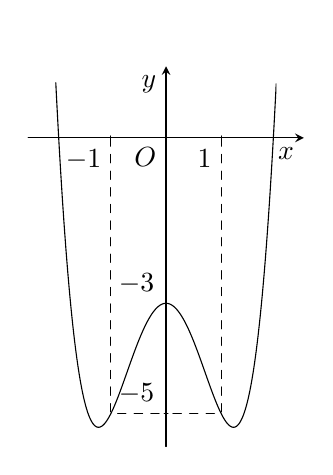
\begin{tikzpicture}[scale=.7, line join=round, line cap=round,>=stealth]

		\tikzset{label style/.style={font=\footnotesize}}

		\draw[->] (-2.5,0)--(2.5,0) node[below left] {$x$};
		\draw[->] (0,-5.6)--(0,1.3) node[below left] {$y$};
		\draw (0,0) node [below left] {$O$};
		\foreach \x in {-1,1}
		\draw[thin] (\x,1pt)--(\x,-1pt) node [below left] {$\x$};
		\foreach \y in {-3,-5}
		\draw[thin] (1pt,\y)--(-1pt,\y) node [above left] {$\y$};
		\draw[dashed,thin](-1,0)--(-1,-5)--(0,-5);
		\draw[dashed,thin](1,0)--(1,-5)--(0,-5);
		\begin{scope}
		\clip (-2.2,-5.5) rectangle (2,2);
		\draw[samples=200,domain=-2:2,smooth,variable=\x] plot (\x,{1*((\x)^4)+0*((\x)^3)+-3*((\x)^2)+0*(\x)-3});
		\end{scope}
	\end{tikzpicture}}
	\loigiai{
		Xét phương trình $x^4-3x^2+m=0\Leftrightarrow x^4-3x^2-3=-m-3$.\\
		Khi đó dựa vào đồ thị để phương trình đã cho có ba nghiệm thì $-m-3=-3\Leftrightarrow m=0$.}
\end{ex}
\begin{ex}%[2D1Y2-2]
	\immini{Cho hàm số $y=f(x)$ có bảng biến thiên như hình vẽ bên. Mệnh đề nào dưới đây đúng?
	\choice
	{$y_{\text{CT}}=0$}
	{$\max\limits_{\mathbb{R}} y=5$}
	{\True $y_{\text{CĐ}}=5$}
	{$\min\limits_{\mathbb{R}} y=4$}}
	{{
\begin{tikzpicture}[scale=.9]
			\tkzTabInit[espcl=1.5,lgt=1.5,nocadre]
			{$x$/0.7,$y'$/0.7,$y$/1.7}
			{$-\infty$,$0$,$1$,$+\infty$}
			\tkzTabLine{,-,0,+,d,-,}
			\tkzTabVar{+/$+\infty$,-/$4$,+/$5$,-/$-\infty$}
			\end{tikzpicture}}}
	
	\loigiai{
		Dựa vào bảng biến thiên ta thấy hàm số đạt cực đại tại $x=1$,; đạt cực tiểu tại $x=0$, $y_{\text{CT}}=4$; hàm số không có giá trị lớn nhất và giá trị nhỏ nhất.}
\end{ex}
\begin{ex}%[2D1Y4-1]
	Tìm đường tiệm cận đứng và đường tiệm cận ngang của đồ thị hàm số $y=\dfrac{2x-1}{x+1}$. 
	\choice
	{$x=\dfrac{1}{2}, y=-1$}
	{$x=1, y=-2$}
	{\True $x=-1, y=2$}
	{$x=-1, y=\dfrac{1}{2}$}
	\loigiai{		
		Ta có:\\
		Vì $\lim\limits_{x\to\pm\infty}\dfrac{2x-1}{x+1}=\lim\limits_{x\to\pm\infty}\dfrac{2-\dfrac{1}{x}}{1+\dfrac{1}{x}}=2$ nên đường thẳng $y=2$ là tiệm cận ngang của đồ thị hàm số.\\
		Vì $\lim\limits_{x\to-1^+}\dfrac{2x-1}{x+1}=-\infty$, $\lim\limits_{x\to-1^-}\dfrac{2x-1}{x+1}=+\infty$ nên đường thẳng $x=-1$ là tiệm cân đứng của đồ thị hàm số.}
\end{ex}
\begin{ex}%[2D1Y1-1]
	Các khoảng đồng biến của hàm số $y=x^3+3x$ là
	\choice
	{$(0;+\infty)$}
	{$(0;2)$}
	{\True $\mathbb{R}$}
	{$(-\infty;1)$ và $(2;+\infty)$}
	\loigiai{
		$y'=3x^2+3>0\forall x\in\mathbb{R}$ suy ra hàm số đồng biến trên $\mathbb{R}$.}
\end{ex}
\begin{ex}%[1D5B2-2]
	Cho hàm số $y=\dfrac{x-1}{x+2}$ có đồ thị $(H)$. Tiếp tuyến của $(H)$ tại giao điểm của $(H)$ với trục hoành có phương trình là 
	\choice
	{$y=3x$}
	{$y=x-3$}
	{$y=3x-3$}
	{\True $y=\dfrac{1}{3}(x-1)$}
	\loigiai{
		Phương trình hoành độ giao điểm của $(H)$ và trục hoành $\dfrac{x-1}{x+2}=0\Leftrightarrow x=1$.\\
		Giao điểm của $(H)$ và trục hoành là $M(1;0)$.\\
		Ta có $y'=\dfrac{3}{(x+2)^2},\forall x\neq-2$.\\
		Phương trình tiếp tuyến của $(H)$ tại $M(1;0)$ là $y=y'(1)\cdot (x-1)=\dfrac{1}{3}(x-1)$.}
\end{ex}
\begin{ex}%[2D1Y2-2]
	\immini{Cho hàm số $y=f(x)$ có đồ thị như hình bên. Mệnh đề nào dưới đây đúng?
	\choice
	{Hàm số có giá trị cực tiểu bằng $2$}
	{\True Hàm số đạt cực đại tại $x=0$ và đạt cực tiểu tại $x=2$}
	{Hàm số có giá trị lớn nhất bằng $2$ và giá trị nhỏ nhất bằng $-2$}
	{Hàm số có ba điểm cực trị}}
	{\begin{tikzpicture}[scale=.7, line join=round, line cap=round,>=stealth]

		\tikzset{label style/.style={font=\footnotesize}}

		\draw[->] (-1.5,0)--(3.5,0) node[below left] {$x$};
		\draw[->] (0,-3.1)--(0,3) node[below left] {$y$};
		\draw (0,0) node [below left] {$O$};
		\foreach \x in {2}
		\draw[thin] (\x,1pt)--(\x,-1pt) node [below left] {$\x$};
		\foreach \y in {-2}
		\draw[thin] (1pt,\y)--(-1pt,\y) node [left] {$\y$};
		\draw[dashed,thin](2,0)--(2,-2)--(0,-2);
		\begin{scope}
		\clip (-3.5,-3) rectangle (3.5,3.5);
		\draw[samples=200,domain=-1.1:3,smooth,variable=\x] plot (\x,{1*((\x)^3)+-3*((\x)^2)+0*(\x)+2});
		\end{scope}
		\end{tikzpicture}}
	\loigiai{
		Dựa vào đồ thị ta thấy hàm số có $2$ cực trị.\\
		Hàm số đạt cực đại tại $x=0$ và giá trị cực đại bằng $2$.\\
		Hàm số đạt cực tiểu tại $B(1;-1)$ và giá trị cực tiểu bằng $-2$.}
\end{ex}
\begin{ex}%[2D1Y2-1]
	Số cực trị của hàm số $y=x^4+2x^2-3$ là
	\choice
	{$0$}
	{$2$}
	{$3$}
	{\True $1$}
	\loigiai{
		Tập xác định $\mathscr{D}=\mathbb{R}$.\\
		$y'=4x^3+4x=4x\left(x^2+1\right)$.\\
		$y'=0\Leftrightarrow x=0\Rightarrow y=-3$.\\
		$y''=12x^2+4$.\\
		$y''(0)=4>0\Rightarrow$ hàm số có một cực tiểu.\\
		Vậy hàm số có một cực trị.}
\end{ex}
\begin{ex}%[2D1K4-3].
	Gọi (H) là đồ thị hàm số $y=\dfrac{2x+3}{x+1}$. Điểm $M(x_0;y_0)$ thuộc (H) có tổng khoảng cách đến hai đường tiệm cận là nhỏ nhất, với $x_0<0$ khi đó $x_0+y_0$ bằng
	\choice
	{$-2$}
	{\True $-1$}
	{$0$}
	{$3$}
	\loigiai{
		Tập xác định. $\mathbb{R}\setminus\{-1\}$.\\
		Dễ có tiệm cận đứng $d_1\colon x=-1$ và tiệm cận ngang $d_2\colon y=2$.\\
		Ta có $\mathrm{d}(M, d_1)+\mathrm{d}(M, d_2)=|x_0+1|+\left|\dfrac{2x_0+3}{x_0+1}-1\right|=|x_0+1|+\left|\dfrac{1}{x_0+1}\right|\geq 2$.\\
		Đẳng thức xảy ra khi và chỉ khi $|x_0+1|=\left|\dfrac{1}{x_0+1}\right|\Leftrightarrow x_0=0\vee x_0=-2$. Vì $x_0<0$ nên $x_0=-2\Rightarrow y_0=1\Rightarrow x_0+y_0=-1$.}
\end{ex}
\begin{ex}%[2D1B3-6]
	Một chất điểm chuyển động có phương trình chuyển động là $s=-t^3+6t^2+17t$, với $t(s)$ là khoảng thời gian tính từ lúc vật bắt đầu chuyển động và $s(m)$ là quãng đường vật đi được trong khoảng thời gian đó. Trong khoảng thời gian 8 giây đầu tiên, vận tốc $v(\mathrm{m/s})$ của chất điểm đạt giá trị lớn nhất bằng
	\choice
	{\True $29 \;\mathrm{m/s}$}
	{$26\;\mathrm{m/s}$}
	{$17\;\mathrm{m/s}$}
	{$36\;\mathrm{m/s}$}
	\loigiai{
		Có: $v=s'=-3t^2+12t+17$.\\
		Ta đi tìm giá trị lớn nhất của $v=-3t^2+12t+17$ trên khoảng $(0;8)$.\\
		$v'=-6t^2+12$, $v'=0\Rightarrow t=2$.\\
		BBT:
		\begin{center}
			
\begin{tikzpicture}[scale=.9]
			\tkzTabInit[espcl=2.5,lgt=1.5,nocadre]
			{$t$/0.7,$v'$/0.7,$v$/1.7}
			{$0$,$2$,$8$}
			\tkzTabLine{,+,0,-,}
			\tkzTabVar{-/,+/$29$,-/}
			\end{tikzpicture}
		\end{center}
		Vậy vận tốc lớn nhất trong khoảng 8 giây đầu tiên là $29\;\mathrm{m/s}$.}
\end{ex}
\begin{ex}%[2D1B5-1]
	\immini{Cho hàm số $y=f(x)=ax^3+bx^2+cx+d$ có đồ thị như hình vẽ ở bên. Mệnh đề nào.
	\choice
	{$a>0$, $b>0$, $c<0$, $d>0$}
	{$a>0$, $b>0$, $c>0$, $d>0$}
	{\True $a>0$, $b<0$, $c>0$, $d>0$}
	{$a<0$, $b<0$, $c>0$, $d<0$}}
	{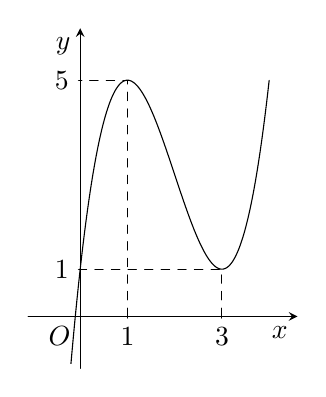
\begin{tikzpicture}[scale=.6, line join=round, line cap=round,>=stealth]

		\tikzset{label style/.style={font=\footnotesize}}

		\draw[->] (-1.1,0)--(4.6,0) node[below left] {$x$};
		\draw[->] (0,-1.1)--(0,6.1) node[below left] {$y$};
		\draw (0,0) node [below left] {$O$};
		\foreach \x in {1,3}
		\draw[thin] (\x,1pt)--(\x,-1pt) node [below] {$\x$};
		\foreach \y in {1,5}
		\draw[thin] (1pt,\y)--(-1pt,\y) node [left] {$\y$};
		\draw[dashed,thin](1,0)--(1,5)--(0,5);
		\draw[dashed,thin](3,0)--(3,1)--(0,1);
		\begin{scope}
		\clip (-1,-1) rectangle (4.5,6);
		\draw[samples=200,domain=-0.2:4,smooth,variable=\x] plot (\x,{1*((\x)^3)+-6*((\x)^2)+9*(\x)+1});
		\end{scope}
		\end{tikzpicture}}
	\loigiai{
		Ta có $y'=3ax^2+2bx+c$.\\
		Dựa vào đồ thị ta thấy nhánh cuối cùng bên phải hướng lên trên suy ra $a>0$.\\
		Đồ thị cắt trục tung tại điểm $x=1\Rightarrow d=1>0$.\\
		Hàm số có 2 điểm cực trị $x_1=1>0$, $x_2=3>0\Rightarrow x_1+x_2>0\Rightarrow-\dfrac{2b}{3a}>0\Rightarrow b<0$.\\
		$x_1x_2>0\Rightarrow\dfrac{c}{3a}>0\Rightarrow c>0$.\\
		Vậy $a>0$, $b<0$, $c>0$, $d>0$.}
\end{ex}
\begin{ex}%[2D1K4-2] 
	Phương trình đường tiệm cận ngang của đồ thị hàm số $y=2x+m-\sqrt{4x^2+x+1}$ (với m là tham số) là
	\choice
	{$y=\dfrac{4m+1}{4}$}
	{\True $y=\dfrac{4m-1}{4}$}
	{$y=\dfrac{2m+1}{2}$}
	{$y=\dfrac{2m-1}{2}$}
	\loigiai{
		Ta có:\\
		• $\lim\limits_{x\to+\infty}\left(2x+m-\sqrt{4x^2+x+1}\right) =\lim\limits_{x\to+\infty}\dfrac{(2x+m)^2-\left(4x^2+x+1\right)}{2x+m+\sqrt{4x^2+x+1}} =\lim\limits_{x\to+\infty}\dfrac{(4m-1)x+m^2-1}{2x+m+\sqrt{4x^2+x+1}}$.\\
		$=\lim\limits_{x\to+\infty}\dfrac{(4m-1)+\dfrac{m^2-1}{x}}{2+\dfrac{m}{x}+\sqrt{4+\dfrac{1}{x}+\dfrac{1}{x^2}}} =\dfrac{4m-1}{4}$.\\
		• $\lim\limits_{x\to-\infty}\left(2x+m-\sqrt{4x^2+x+1}\right)$.\\
		$=\lim\limits_{x\to-\infty} x\left(2+\dfrac{m}{x}+\sqrt{4+\dfrac{1}{x}+\dfrac{1}{x^2}}\right)=-\infty$.\\
		Suy ra đồ thị hàm số có một đường tiệm cận ngang là $y=\dfrac{4m-1}{4}$.}
\end{ex}
\begin{ex}%[2D1K3-1]
	Tìm tất cả các giá trị thực của tham số $m$ để giá trị nhỏ nhất của hàm số $y=\dfrac{x+2m^2-m}{x-3}$ trên đoạn $[0;1]$ bằng $-2$. 
	\choice
	{$m=1$ hoặc $m=-\dfrac{1}{2}$}
	{$m=3$ hoặc $m=-\dfrac{5}{2}$}
	{\True $m=-1$ hoặc $m=\dfrac{3}{2}$}
	{$m=2$ hoặc $m=-\dfrac{3}{2}$}
	\loigiai{
		$y=\dfrac{x+2m^2-m}{x-3}\Rightarrow y'=\dfrac{-3-2m^2+m}{(x-3)^2}<0$ \\
		$ \Rightarrow y_{\min} =y_{(1)}=\dfrac{2m^2-m+1}{-2} $ \\
		$ \Rightarrow y_{\min} =-2\Leftrightarrow\dfrac{2m^2-m+1}{-2}=-2\Leftrightarrow 2m^2-m+1=4 $ \\
		$ \Leftrightarrow 2m^2-m-3-0\Leftrightarrow\hoac{&m=-1\\&m=\dfrac{3}{2}} $.}
\end{ex}
\begin{ex}%[2D1B1-1]
	Hàm số $y=\sqrt{8+2x-x^2}$ đồng biến trên khoảng nào sau đây?
	\choice
	{$(1;+\infty)$}
	{$(1; 4)$}
	{$(-\infty; 1)$}
	{\True $(-2; 1)$}
	\loigiai{
		Xét hàm số: $y=\sqrt{8+2x-x^2}$ có:\\
		TXĐ: $\mathscr{D}=[-2; 4]$.\\
		$y'=\dfrac{\left(8+2x-x^2\right)'}{2\sqrt{8+2x-x^2}}=\dfrac{2-2x}{2\sqrt{8+2x-x^2}}=\dfrac{1-x}{\sqrt{8+2x-x^2}}$; $y'=0\Leftrightarrow x=1$.\\
		Ta có bảng biến thiên: 
		\begin{center}
			
\begin{tikzpicture}[scale=.9]
				\tkzTabInit[espcl=2.5,lgt=1.5,nocadre]
				{$x$/0.7,$y'$/0.7,$y$/1.7}
				{$-2$,$1$,$4$}
				\tkzTabLine{,+,0,-,}
				\tkzTabVar{-/$0$,+/$3$,-/$0$}
			\end{tikzpicture}
		\end{center}
		Dựa vào bảng biến thiên ta có hàm số $y=\sqrt{8+2x-x^2}$ đồng biến trên khoảng $(-2; 1)$.}
\end{ex}
\begin{ex}%[2D1B1-3]
	Tìm tất cả các giá trị thực của tham số $m$ để hàm số $y=\dfrac{2x-m}{x-1}$ đồng biến trên khoảng xác định của nó. 
	\choice
	{$m\in(1; 2)$}
	{$m\in[2;+\infty)$}
	{\True $m\in(2;+\infty)$}
	{$m\in(-\infty; 2)$}
	\loigiai{
		TXĐ: $\mathscr{D}=\mathbb{R}\setminus\{1\}$.\\
		Ta có $y'=\dfrac{m-2}{(x-1)^2}$. Để hàm số đồng biến trên khoảng xác định của nó thì $y'>0\Leftrightarrow\dfrac{m-2}{(x-1)^2}>0\forall x\in \mathscr{D}\Leftrightarrow m>2$ suy ra $m\in(2;+\infty)$.}
\end{ex}
\begin{ex}%[2D1B2-2]
	Gọi $A$, $B$ là các giao điểm của đồ thị hàm số $y=\dfrac{2x+1}{x+1}$ và đường thẳng $y=-x-1$. Tính $AB$. 
	\choice
	{\True $AB=4$}
	{$AB=\sqrt{2}$}
	{$AB=2\sqrt{2}$}
	{$AB=4\sqrt{2}$}
	\loigiai{
		Tọa độ các điểm $A$, $B$ là nghiệm của hệ phương trình:\\
		$f(x)\Leftrightarrow\heva{&y=-x-1\\&x^2+4x+2=0}\Leftrightarrow\heva{&y=-x-1\\&x=-2\pm\sqrt{2}}\Rightarrow\heva{&A\left(-2-\sqrt{2};1+\sqrt{2}\right)\\&B\left(-2+\sqrt{2};1-\sqrt{2}\right)}$ \\
		$ \Rightarrow\overrightarrow{AB}=\left(2\sqrt{2};-2\sqrt{2}\right)\Rightarrow AB=4 $.}
\end{ex}
\begin{ex}%Câu 21.%[2D1Y2-2]
	\immini{Cho hàm số $y=f(x)$ xác định trên $\mathbb{R}$ và có đồ thị hàm số $y=f'(x)$ là đường cong ở hình bên. Hỏi hàm số $y=f(x)$ có bao nhiêu điểm cực trị?
	\choice
	{$6$}
	{$5$}
	{$4$}
	{\True $3$}}
	{\begin{tikzpicture}[line join=round, line cap=round,>=stealth]

		\tikzset{label style/.style={font=\footnotesize}}

		\draw[->] (-2.1,0)--(1.6,0) node[below left] {$x$};
		\draw[->] (0,-1.1)--(0,3.1) node[below left] {$y$};
		\draw (0,0) node [below left] {$O$};
		\begin{scope}
		\clip (-2,-1) rectangle (1.5,3);
		\draw[name path=c] plot[smooth,tension=.8] coordinates{(0.96, -0.34)  (0.4,2.5) (-0.5,0.1) (-0.88,0.74) (-1.2,-0.48) (-1.48,2.34)};
		\end{scope}
		\end{tikzpicture}}
	\loigiai{
		Dựa vào đồ thị $y=f'(x)$ ta thấy phương trình $f'(x)=0$ có 4 nghiệm nhưng giá trị $f'(x)$ chỉ đổi dấu 3 lần.\\
		Vậy hàm số $y=f(x)$ có 3 điểm cực trị.}
%<MyLT>
\end{ex}
\begin{ex}%[2D1B2-3]
	Tìm tất cả các giá trị thực của tham số $m$ để hàm số $y=mx^3+x^2+\left(m^2-6\right)x+1$ đạt cực tiểu tại $x=1$. 
	\choice
	{\True $m=1$}
	{$m=-4$}
	{$m=-2$}
	{$m=2$}
	\loigiai{
		Ta có: $y'=3mx^2+2x+m^2-6$ và $y''=6mx+2$.\\
		Để hàm số $y=mx^3+x^2+\left(m^2-6\right)x+1$ đạt cực tiểu tại $x=1$ thì: $\heva{&y'(1)=0\\&y''(1)>0}\Leftrightarrow\heva{&m^2+3m-4=0\\&6m+2>0}\Leftrightarrow\heva{&\hoac{&m=1\\&m=-4}\\&m >-\dfrac{1}{3}}\Leftrightarrow m=1$.\\
		Thử lại: với $m=1$ ta có: $y=x^3+x^2-5x+1\Rightarrow y'=3x^2+2x-5$, $y'=0\Leftrightarrow\hoac{&x=1\\&x=-\dfrac{5}{3}.}$ \\
		Vì $a=1>0$ nên hàm số đạt cực đại tại $x=-\dfrac{5}{3}$ và đạt cực tiểu tại $x=1$. Vậy $m=1$ thỏa mãn.}
\end{ex}
\begin{ex}%[2D1K3-6] 
	\immini{Tính diện tích lớn nhất $S_{\max}$ của một hình chữ nhật nội tiếp trong nửa đường tròn bán kính $R=6 \;\mathrm{cm}$ nếu một cạnh của hình chữ nhật nằm dọc theo đường kính của hình tròn mà hình chữ nhật đó nội tiếp.} 
	{\begin{tikzpicture}[scale=.8, line join=round, line cap=round,>=stealth]
		\tikzset{label style/.style={font=\footnotesize}}
		\draw[name path=v] (3,0) arc (0:180:3cm);
		\coordinate (M) at (-3,0);
		\coordinate (N) at (3,0);
		\draw[name path=MN] (M)--(N);
		\coordinate (O) at (0,0);
		\coordinate (C) at (2,0);
		\coordinate (D) at (-2,0);
		\coordinate (A) at (-2,2.236);
		\coordinate (B) at (2,2.236);
		\tkzDrawSegments(A,B B,C C,D D,A)
		\tkzDrawPoints[fill=black,size=2pt](A,B,C,D)
		\tkzFillPolygon[pattern=north east lines](A,B,C,D)
		\end{tikzpicture}}
	\choice
	{$S_{\max} =36\pi \;\mathrm{cm}^2$}
	{\True $S_{\max} =36 \;\mathrm{cm}^2$}
	{$S_{\max} =96\pi \;\mathrm{cm}^2$}
	{$S_{\max} =18 \;\mathrm{cm}^2$}
	\loigiai{
		\immini{Gọi hình chữ nhật cần tính diện tích là $ABCD$ có $OC=x (0<x<6)$, $OB=6$.\\
		Khi đó diện tích của hình chữ nhật $ABCD$ là $S=AB\cdot BC =2x\sqrt{36-x^2} =f(x)$.}
		{\begin{tikzpicture}[scale=.8, line join=round, line cap=round,>=stealth]
			\tikzset{label style/.style={font=\footnotesize}}
			\draw[name path=v] (3,0) arc (0:180:3 cm);
			\coordinate (M) at (-3,0);
			\coordinate (N) at (3,0);
			\draw[name path=MN] (M)--(N);
			\coordinate (O) at (0,0);
			\coordinate (C) at (2,0);
			\coordinate (D) at (-2,0);
			\coordinate (A) at (-2,2.236);
			\coordinate (B) at (2,2.236);
			\tkzDrawSegments(A,B B,C C,D D,A)
			\tkzDrawPoints[fill=black,size=2pt](A,B,C,D,O)
			\coordinate (x) at ($(O)!0.5!(C)$);
			\tkzLabelPoints[below](O,C,D,x)
			\tkzLabelPoints[above left](A)
			\tkzLabelPoints[above right](B)
			\tkzFillPolygon[pattern=north east lines](A,B,C,D)
			\end{tikzpicture}}
		\noindent Diện tích lớn nhất của hình chữ nhật $ABCD$ là giá trị lớn nhất của $f(x) =2x\sqrt{36-x^2}$ trên $(0; 6)$.\\
		$f'(x)=2\sqrt{36-x^2}-\dfrac{2x^2}{\sqrt{36-x^2}} =\dfrac{-4x^2+72}{\sqrt{36-x^2}}$.\\
		$f'(x)=0\Leftrightarrow\hoac{&x=3\sqrt{2}\in(0; 6)\\&x=-3\sqrt{2}\notin(0; 6).}$ \\
		$BBT$ 
		\begin{center}
			
\begin{tikzpicture}[scale=.9]
			\tkzTabInit[espcl=2.5,lgt=1.5,nocadre]
			{$x$/0.7,$f'(x)$/0.7,$f(x)$/1.7}
			{$0$,$3\sqrt 2$,$6$}
			\tkzTabLine{,+,0,-,}
			\tkzTabVar{-/$0$,+/$36$,-/$0$}
			\end{tikzpicture}
		\end{center}
		Ta có: $\max\limits_{(0; 6)} f(x)=36$.\\
		Vậy $S_{\max} =36 \;\mathrm{cm}^2$.}
\end{ex}
\begin{ex}%[2D1B5-2]
	\immini{Cho hàm số $y=f(x)$ có đồ thị trong hình vẽ bên. Tìm tất cả các giá trị của $m$ để phương trình $\left|f(x)\right|=m$ có đúng hai nghiệm phân biệt.
	\choice
	{\True $m>5$, $0<m<1$}
	{$m<1$}
	{$m=1$, $m=5$}
	{$1<m<5$}}
	{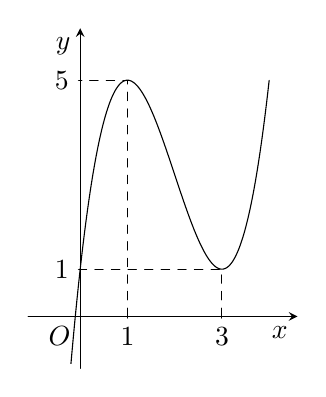
\begin{tikzpicture}[scale=.6, line join=round, line cap=round,>=stealth]		
		\tikzset{label style/.style={font=\footnotesize}}		
		\draw[->] (-1.1,0)--(4.6,0) node[below left] {$x$};
		\draw[->] (0,-1.1)--(0,6.1) node[below left] {$y$};
		\draw (0,0) node [below left] {$O$};
		\foreach \x in {1,3}
		\draw[thin] (\x,1pt)--(\x,-1pt) node [below] {$\x$};
		\foreach \y in {1,5}
		\draw[thin] (1pt,\y)--(-1pt,\y) node [left] {$\y$};
		\draw[dashed,thin](1,0)--(1,5)--(0,5);
		\draw[dashed,thin](3,0)--(3,1)--(0,1);
		\begin{scope}
		\clip (-1,-1) rectangle (4.5,6);
		\draw[samples=200,domain=-0.2:4,smooth,variable=\x] plot (\x,{1*((\x)^3)+-6*((\x)^2)+9*(\x)+1});
		\end{scope}
		\end{tikzpicture}}
	\loigiai{
		\immini{Từ đồ thị $(C)$ của hàm số $y=f(x)$ ta suy ra đồ thị $(C')$ của hàm số $y=\left|f(x)\right|$ như sau:\\
		- Giữ nguyên phần đồ thị $(C)$ ở phía trên trục hoành.\\
		- Lấy đối xứng qua trục hoành phần đồ thị $(C)$ ở phía dưới trục hoành.\\
		Khi đó, đồ thị $(C')$ là hợp của hai phần trên.\\
		Ta có: $\left|f(x)\right|=m$ là phương trình hoành độ giao điểm của đồ thị $(C')$ và đường thẳng $(d)\colon y=m$ (song song hoặc trùng với trục hoành).}
		{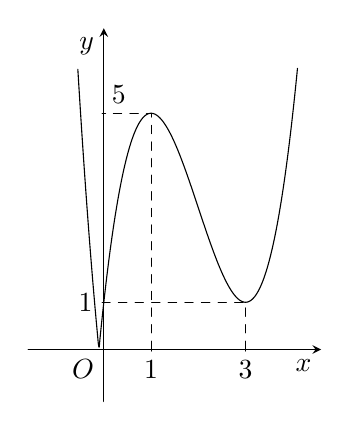
\begin{tikzpicture}[scale=.6, line join=round, line cap=round,>=stealth]			
			\tikzset{label style/.style={font=\footnotesize}}			
			\draw[->] (-1.6,0)--(4.6,0) node[below left] {$x$};
			\draw[->] (0,-1.1)--(0,6.8) node[below left] {$y$};
			\draw (0,0) node [below left] {$O$};
			\foreach \x in {1,3}
			\draw[thin] (\x,1pt)--(\x,-1pt) node [below] {$\x$};
			\foreach \y in {1}
			\draw[thin] (1pt,\y)--(-1pt,\y) node [left] {$\y$};
			\draw[thin] (1pt,5)--(-1pt,5) node [above right] {$5$};
			\draw[dashed,thin](1,0)--(1,5)--(0,5);
			\draw[dashed,thin](3,0)--(3,1)--(0,1);
			\begin{scope}
			\clip (-1,-1) rectangle (4.5,6);
			\draw[samples=300,domain=-0.55:4.1,smooth,variable=\x] plot (\x, {abs(1*((\x)^3)+-6*((\x)^2)+9*(\x)+1)});
			\end{scope}
			\end{tikzpicture}}
		\noindent Dựa vào đồ thị $(C')$, ta có phương trình $\left|f(x)\right|=m$ có đúng hai nghiệm phân biệt khi và chỉ khi $\hoac{&0<m<1\\&m>5}$.}
\end{ex}
\begin{ex}%[2D1B5-1]
	\immini{Cho hàm số $y=\dfrac{x-a}{bx+c}$ có đồ thị như hình vẽ bên dưới. Tính giá trị của biểu thức $P=a+b+c$.
	\choice
	{\True $P=-3$}
	{$P=1$}
	{$P=5$}
	{$P=2$}} 
	{\begin{tikzpicture}[scale=.5, line join=round, line cap=round,>=stealth]

		\tikzset{label style/.style={font=\footnotesize}}

		\draw[->] (-5.1,0)--(6.1,0) node[below left] {$x$};
		\draw[->] (0,-5.1)--(0,6.1) node[below left] {$y$};
		\draw (0,0) node [below right] {$O$};
		\foreach \x in {-2}
		\draw[thin] (\x,1pt)--(\x,-1pt) node [below left] {$\x$};
		\draw[thin] (2,1pt)--(2,-1pt) node [below right] {$2$};
		\foreach \y in {-1}
		\draw[thin] (1pt,\y)--(-1pt,\y) node [below left] {$\y$};
		\draw[thin] (1pt,1)--(-1pt,1) node [above left] {$1$};
		\draw[dashed,thin] (2.01,-5)--(2.01,6);
		\begin{scope}
		\clip (-5,-5) rectangle (6,6);
		\draw[samples=200,domain=-5:1.99,smooth,variable=\x] plot (\x,{(1*(\x)+2)/(1*(\x)+-2)});
		\draw[samples=200,domain=2.01:6,smooth,variable=\x] plot (\x,{(1*(\x)+2)/(1*(\x)+-2)});
		\draw[dashed,thin] (-5,1/1)--(6,1/1);
		\end{scope}
		\end{tikzpicture}}
	\loigiai{
		Ta có: Tiệm cận đứng: $x=2\Rightarrow-\dfrac{c}{b}=2\Leftrightarrow 2b+c=0 (1)$.\\
		Tiệm cận ngang: $y=1\Rightarrow\dfrac{1}{b}=1\Leftrightarrow b=1 (2)$.\\
		Thế $(2)$ vào $(1)$ suy ra $c=-2$. Suy ra hàm số có dạng $y=\dfrac{x-a}{x-2}$.\\
		Đồ thị hàm số đi qua điểm $(-2;0)$ nên ta có: $0=\dfrac{-2-a}{-2-2}\Leftrightarrow a=-2$.\\
		Vậy $P=-2+1-2 =-3$.}
\end{ex}
\Closesolutionfile{ans}
\begin{center}
	\textbf{Đề số 1}
\end{center}

\Opensolutionfile{ans}[ans/ansCD2D1-6-2]
\begin{ex}%[Nguyễn Tâm Phục]%[2D1B5-4]%Câu 26.
	Tìm tất cả các giá trị thực của tham số $m$ để đường thẳng $y=m$ cắt đồ thị hàm số $y=x^4-2x^2$ tại $4$ điểm phân biệt. 
	\choice
	{\True $-1<m<0$}
	{$m<0$}
	{$0<m<1$}
	{$m>0$}
	\loigiai{
		Tập xác định $\mathscr{D}=\mathbb{R}$.\\
		$y'=4x^3-4x$, $y'=0\Leftrightarrow\hoac{&x=0\Rightarrow y=0\\&x=\pm 1\Rightarrow y=-1.}$ \\
		Bảng biến thiên
		\begin{center}
			
\begin{tikzpicture}
			\tkzTabInit[espcl=2.3,lgt=1.3]
			{$x$/0.7,$y'$/0.7,$y$/2.1}
			{$-\infty$,$-1$,0,$1$,$+\infty$}
			\tkzTabLine{,+,0,-,0,+,0,-}
			\tkzTabVar{-/$-\infty$,+/$-1$,-/$0$,+/$-1$,-/$-\infty$}
			\end{tikzpicture}
		\end{center}
		Dựa vào bảng biến thiên ta có giá trị $m$ cần tìm là $-1<m<0$.}
\end{ex}
\begin{ex}%[Nguyễn Tâm Phục]%[2D1K1-3]%Câu 27.
	Tìm tất cả giá trị thực của tham số $m$ để hàm số $y=\dfrac{1}{3}x^3-2mx^2+4x-5$ đồng biến trên $\mathbb{R}$. 
	\choice
	{$-1<m<1$}
	{\True $-1\leq m\leq 1$}
	{$0\leq m\leq 1$}
	{$0<m<1$}
	\loigiai{
		Tập xác định: $\mathscr{D}=\mathbb{R}$.\\
		Đạo hàm: $y'=x^2-4mx+4$.\\
		Hàm số đã cho đồng biến trên tập xác định $\mathbb{R}$ khi và chỉ khi $y'\geq 0,\forall x\in\mathbb{R}$ và dấu “=” chỉ xảy ra tại hữu hạn điểm trên $\mathbb{R}$.\\
		Điều kiện: $\Delta'=4m^2-4\leq 0$, $\forall m\in\mathbb{R}\Leftrightarrow-1\leq m\leq 1$.}
\end{ex}
\begin{ex}%[Nguyễn Tâm Phục]%[2D1B2-3]%Câu 28.
	Tìm giá trị thực của tham số $m$ để hàm số $y=\dfrac{1}{3}x^3-mx^2+\left(m^2-m-1\right)x$ đạt cực đại tại $x=1$. 
	\choice
	{$m=2$}
	{\True $m=3$}
	{$m\in\emptyset$}
	{$m=0$}
	\loigiai{
		Tập xác định $\mathscr{D}=\mathbb{R}$.\\
		Ta có: $y'=x^2-2mx+m^2-m-1$; $y''=2x-2m$.\\
		Hàm số đạt cực đại tại $x=1$ suy ra $y'(1)=0\Leftrightarrow m^2-3m=0\Leftrightarrow\hoac{&m=0\\&m=3.}$ \\
		+ Với $m=0$: $y''(1)=2>0\Rightarrow x=1$ là điểm cực tiểu của hàm số.\\
		+  Với $m=3$: $y''(1)=-4<0\Rightarrow x=1$ là điểm cực đại của hàm số.\\
		Vậy $m=3$ là giá trị cần tìm.}
\end{ex}
\begin{ex}%[Nguyễn Tâm Phục]%[2D1K1-3]%Câu 29.
	Gọi $S$ là tập hợp các giá trị của tham số $m$ để hàm số $y=\dfrac{1}{3}x^3-\dfrac{1}{2}mx^2+2mx-3m+4$ nghịch biến trên một đoạn có độ dài bằng $3$. Tính tổng tất cả phần tử của $S$. 
	\choice
	{$9$}
	{$-1$}
	{$-8$}
	{\True $8$}
	\loigiai{
		TXĐ: $\mathscr{D}=\mathbb{R}$.\\
		Ta có: $y'=x^2-mx+2m$, $y'=0\Leftrightarrow x^2-mx+2m=0$ (1).\\
		Để hàm số đã cho nghịch biến trên một đoạn có độ dài bằng $3$ thì $(1)$ phải có hai nghiệm $x_1$, $x_2$ thỏa mãn $|x_1-x_2|=3$. Điều này tương đương với.\\
		$\heva{&\Delta'>0\\&|x_1-x_2|=3}\Leftrightarrow\heva{&m^2-8m>0\\&m^2-8m-9=0}\Leftrightarrow\hoac{&m=-1\\&m=9.}$ \\
		Do đó, $S=\{-1; 9\}$.\\
		Vậy tổng tất cả các phần tử của $S$ là $8$.}
\end{ex}
\begin{ex}%[Nguyễn Tâm Phục]%[2D1K5-4]%Câu 30.
	Tổng bình phương các giá trị của tham số $m$ để đường thẳng $(d)\colon y=-x+m$ cắt đồ thị $(C)\colon y=\dfrac{-2x+1}{x+1}$ tại hai điểm phân biệt $A$, $B$ với $AB=2\sqrt{2}$ là
	\choice
	{$84$}
	{$5$}
	{\True $50$}
	{$2$}
	\loigiai{
		Phương trình hoành độ giao điểm của $(d)$ và $(C)$:\\
		\begin{eqnarray*}
			&&\dfrac{-2x+1}{x+1}=-x+m \\
			&\Leftrightarrow &-2x+1=(-x+m)(x+1) \\
			&\Leftrightarrow &x^2-(m+1)x+1-m=0\quad (1). 
		\end{eqnarray*}		
		$(1)$ phải có hai nghiệm phân biệt khác $(-1)$. Điều này tương đương với
		$$\Delta>0\Leftrightarrow m^2+6m-3>0 \quad (*).$$
		Gọi $x_1$, $x_2$ là hai nghiệm của $(1)$. Giả sử $A(x_1;-x_1+m)$, $B(x_2;-x_2+m)$.\\
		Khi đó, ta có:
		\begin{eqnarray*}
			&&AB^2=2(x_1-x_2)^2\\
			& \Leftrightarrow & 2(x_1-x_2)^2=8\\
			&\Leftrightarrow & (x_1+x_2)^2-4x_1x_2=4 \\
			& \Leftrightarrow & m^2+6m-7=0\\
			&\Leftrightarrow & \hoac{&m=1\\&m=-7}  (\text{thỏa mãn } (*)).
		\end{eqnarray*}		
		Vậy tổng bình phương các giá trị của tham số $m$ là $50$.}
\end{ex}
\begin{ex}%[Nguyễn Tâm Phục]%[2D1K5-7]%Câu 31.
	Biết đồ thị $(C_m)$ của hàm số $y=x^4-mx^2+m+2018$ luôn luôn đi qua hai điểm $M$ và $N$ cố định khi $m$ thay đổi. Tọa độ trung điểm $I$ của đoạn thẳng $MN$ là
	\choice
	{$I(1; 2018)$}
	{$I(0; 1)$}
	{$I(0; 2018)$}
	{\True $I(0; 2019)$}
	\loigiai{
		Giả sử $M(x_0; y_0)$ là điểm cố định của họ $(C_m)$. Khi đó
		\begin{eqnarray*}
			&&y_0=x_0^4-mx_0^2+m+2018,\forall m\\
			&\Leftrightarrow & \left(-x_0^2+1\right)m+x_0^4-y_0+2018=0,\forall m \\
			&\Leftrightarrow & \heva{&-x_0^2+1=0\\&x_0^4-y_0+2018=0} \\
			&\Leftrightarrow & \heva{&\hoac{&x_0=1\\&x_0=-1}\\&x_0^4-y_0+2018=0}\\
			&\Leftrightarrow&\hoac{&\heva{&x_0=1\\&y_0=2019}\\&\heva{&x_0=-1\\&y_0=2019}} \\
			&\Leftrightarrow & \hoac{&M(1; 2019)\\&N(-1; 2019).}
		\end{eqnarray*}		
		Suy ra tọa độ trung điểm $I$ của đoạn thẳng $MN$ có tọa độ là $I(0; 2019)$.}
\end{ex}
\begin{ex}%[Nguyễn Tâm Phục]%[2D1B5-3]%Câu 32.
	Cho hàm số $y=f(x)$ xác định, liên tục trên $\mathbb{R}$ và có bảng biến thiên sau: 
	\begin{center}
		
\begin{tikzpicture}
		\tkzTabInit[espcl=2.5,lgt=1.5]
		{$x$/0.7,$y'$/0.7,$y$/2.5}
		{$-\infty$,$-1$,0,$1$,$+\infty$}
		\tkzTabLine{,-,0,+,0,-,0,+}
		\tkzTabVar{+/$+\infty$,-/$-1$,+/$0$,-/$-1$,+/$+\infty$}
		\end{tikzpicture}
	\end{center}
	Tìm tất cả các giá trị thực của tham số $m$ để phương trình $f(x)-1=m$ có đúng hai nghiệm. 
	\choice
	{$m=-2, m\geq-1$}
	{$m>0, m=-1$}
	{\True $m=-2, m >-1$}
	{$-2<m <-1$}
	\loigiai{
		Ta có $f(x)-1=m\Leftrightarrow f(x)=m+1$.\\
		Dựa vào bảng biến thiên, để phương trình có đúng hai nghiệm thì $\hoac{&m+1=-1\\&m+1>0}\Leftrightarrow\hoac{&m=-2\\&m >-1}$.}
\end{ex}
\begin{ex}%[Nguyễn Tâm Phục]%[2D1K1-3]%Câu 33.
	Có bao nhiêu giá trị nguyên của tham số $m$ để hàm số $y=\dfrac{mx+4}{x+m}$ giảm trên khoảng $(-\infty;1)$?
	\choice
	{$2$}
	{Vô số}
	{\True $1$}
	{$0$}
	\loigiai{
		Điều kiện $x\neq-m$.\\
		Do $x\in(-\infty;1)$ nên $m\in(-\infty;-1]$.\\
		Ta có $y'=\dfrac{m^2-4}{(x+m)^2}$.\\
		Để hàm số giảm trên khoảng $(-\infty;1)$ thì $y'<0$ với $x\in(-\infty;1)\Leftrightarrow m^2-4<0\Leftrightarrow-2<m<2$.\\
		Do $m$ nguyên và $m\in(-\infty;-1]$ nên $m=-1$.\\
		Vậy có $1$ giá trị của $m$ thỏa mãn.}
\end{ex}
\begin{ex}%[Nguyễn Tâm Phục]%[2D1G4-3]%Câu 34.
	Tiếp tuyến của đồ thị hàm số $y=\dfrac{4x-3}{2x+1}$ cùng với $2$ tiệm cận tạo thành một tam giác có diện tích bằng 
	\choice
	{$6$}
	{$7$}
	{\True $5$}
	{$4$}
	\loigiai{
		Gọi $M(x_0;y_0)$ là điểm nằm trên đồ thị hàm số, $x_0\neq-\dfrac{1}{2}$.\\
		$y'=\dfrac{10}{(2x+1)^2}$.\\
		Phương trình tiếp tuyến tại $M$ là $$y=f'(x_0)(x-x_0)+y_0\Rightarrow y=\dfrac{10}{(2x_0+1)^2}(x-x_0)+\dfrac{4x_0-3}{2x_0+1}.$$
		Tiệm cận đứng: $x=-\dfrac{1}{2}$, tiệm cận ngang: $y=2$.\\
		Gọi $A$ là giao điểm của tiếp tuyến với tiệm cận đứng\\
		Suy ra $ x_A=-\dfrac{1}{2}\Rightarrow y_A=\dfrac{10}{(2x_0+1)^2}\left(-\dfrac{1}{2}-x_0\right)+\dfrac{4x_0-3}{2x_0+1}=\dfrac{4x_0-8}{2x_0+1}$. \\
		Vậy $A\left(-\dfrac{1}{2};\dfrac{4x_0-8}{2x_0+1}\right)$.\\
		Gọi $B$ là giao điểm của tiếp tuyến với tiệm cận ngang\\
		Suy ra $y_B=2\Rightarrow 2=\dfrac{10}{(2x_0+1)^2}(x_B-x_0)+\dfrac{4x_0-3}{2x_0+1}\Rightarrow x_B=2x_0+\dfrac{1}{2}$. Vậy $B\left(\dfrac{4x_0+1}{2};2\right)$.\\
		Giao điểm 2 tiệm cận là $I\left(-\dfrac{1}{2};2\right)$.\\
		Ta có: $\overrightarrow{IA}=\left(0;-\dfrac{10}{2x_0+1}\right)\Rightarrow IA=\left|\dfrac{10}{2x_0+1}\right|$.\\
		$\overrightarrow{IB}=(2x_0+1;0)\Rightarrow IB=|2x_0+1|$.\\
		Tam giác $IAB$ vuông tại $I$ nên $S_{IAB}=\dfrac{1}{2}IA\cdot IB=\dfrac{1}{2}\left|\dfrac{10}{2x_0+1}\right|\cdot|2x_0+1|=5$.}
\end{ex}
\begin{ex}%[Nguyễn Tâm Phục]%[2D1G2-5]%Câu 35.
	Có bao nhiêu giá trị thực của tham số $m$ để đồ thị hàm số $y=x^4-2mx^2+m-1$ có ba điểm cực trị tạo thành một tam giác có bán kính đường tròn ngoại tiếp chúng bằng $1$?
	\choice
	{\True $1$}
	{$2$}
	{$3$}
	{$4$}
	\loigiai{
		$y'=4x^3-4mx=4x\left(x^2-m\right)$.\\
		Xét $y'=0\Leftrightarrow\hoac{&x=0\\&x=\pm\sqrt{m}} (m>0)$.\\
		Tọa độ ba điểm cực trị là $$A(0; m-1), B\left(-\sqrt{m};-m^2+m-1\right), C\left(\sqrt{m};-m^2+m-1\right).$$
		Gọi $H$ là trung điểm của cạnh $BC$. Ta có $H\left(0;-m^2+m-1\right)$.\\
		$S_{\triangle ABC}=\dfrac{1}{2}AH\cdot BC=\dfrac{AB\cdot AC\cdot BC}{4R}$ (do $\Delta ABC$ cân tại $A$)\\
		Khi và chỉ khi $AB^2=2AH\cdot R $ trong đó $\heva{&AH=m^2\\&AB=\sqrt{m+m^4}.}$ \\
		Suy ra $m+m^4=4m^4\Leftrightarrow 3m^4=m\Leftrightarrow m=\dfrac{1}{\sqrt[3]{3}}$.}
\end{ex}
\begin{ex}%[Nguyễn Tâm Phục]%[2D1G2-5]%Câu 36.
	Cho hàm số $y=x^4-2mx^2-2m^2+m^4$ có đồ thị $(C)$. Biết đồ thị $(C)$ có ba điểm cực trị $A$, $B$, $C$ và $ABDC$ là hình thoi trong đó $D(0;-3)$, $A$ thuộc trục tung. Khi đó $m$ thuộc khoảng nào?
	\choice
	{$m\in\left(\dfrac{9}{5};2\right)$}
	{$m\in\left(-1;\dfrac{1}{2}\right)$}
	{$m\in(2;3)$}
	{\True $m\in\left(\dfrac{1}{2};\dfrac{9}{5}\right)$}
	\loigiai{
		Ta có $y'=4x\left(x^2-m\right)\Rightarrow y'=0\Leftrightarrow\hoac{&x=0\\&x^2=m}$;\\
		Với điều kiện $m>0$ đồ thị hàm số có ba điểm cực trị là $$A\left(0;m^4-2m^2\right);B\left(-\sqrt{m};m^4-3m^2\right);C\left(\sqrt{m};m^4-3m^2\right).$$
		Để $ABDC$ là hình thoi điều kiện là $BC\perp AD$ và trung điểm $I$ của $BC$ trùng với trung điểm $J$ của $AD$. \\
		Do tính đối xứng ta luôn có $BC\perp AD$ nên chỉ cần $I\equiv J$ với $I\left(0; m^4-3m^2\right), J\left(0;\dfrac{m^4-2m^2-3}{2}\right)$.\\
		Điều kiện là $$m^4-2m^2-3=2m^4-6m^2\Leftrightarrow m^4-4m^2+3=0\Leftrightarrow\hoac{&m=1\\&m=\sqrt{3}}\Leftrightarrow m\in\left(\dfrac{1}{2};\dfrac{9}{5}\right).$$}
\end{ex}
\begin{ex}%[Nguyễn Tâm Phục]%[2D1G3-6]%Câu 37.
	\immini{Một công ty muốn làm một đường ống dẫn dầu từ một kho $A$ ở trên bờ biển đến một vị trí $B$ trên một hòn đảo. Hòn đảo cách bờ biển $6$ km. Gọi $C$ là điểm trên bờ sao cho $BC$ vuông góc với bờ biển. Khoảng cách từ $A$ đến $C$ là $9$  km. Người ta cần xác định một vị trí $D$ trên $AC$ để lắp ống dẫn theo đường gấp khúc $ADB$. Tính khoảng cách $AD$ để số tiền chi phí thấp nhất, biết rằng giá để lắp đặt mỗi km đường ống trên bờ là $100.000.000$ đồng và dưới nước là $260.000.000$ đồng. 
		\choice
		{$7$ km}
		{$6$  km} 
		{$7{,}5$ km}
		{\True $6{.}5$  km}
	}{
		\begin{tikzpicture}[line cap=round,line join=round,>=stealth,x=1.0cm,y=1.0cm,scale=1]
		\tkzDefPoints{6/0/A,0/4/B,0/0/C,2.5/0/D}
		\tkzDrawPoints[fill=black,size=3](A,B,C,D)
		\tkzLabelPoints[above](A,B)
		\tkzLabelPoints[above right](C);
		\tkzLabelPoints[above right](D);
		\tkzDrawSegments(A,C B,C B,D);
		\draw [<->,dashed](-0.2,0) -- (-0.2,4);
		\draw [<->,dashed](0,-0.2) -- (6,-0.2);
		\tkzLabelPoint[left](-0.2,2){$6$ km};
		\tkzLabelPoint[below](3,-0.2){$9$ km};
		
		\end{tikzpicture} 
	}
	\loigiai{
		Đặt $AD=x$ km, $x>0$; khi đó $CD=9-x$; $BD=\sqrt{36+(9-x)^2}$.\\
		Giá thành lắp đặt là $$100\cdot 10^6x+\sqrt{36+(9-x)^2}\cdot 260\cdot 10^6=10^7\left[10x+26\sqrt{36+(9-x)^2}\right].$$
		Xét hàm số $f(x)=10x+\sqrt{36+(9-x)^2}\cdot 26 \quad (0<x<9)$.\\
		$f'(x)=10-26\cdot\dfrac{9-x}{\sqrt{36+(9-x)^2}}=0\Leftrightarrow 10\sqrt{36+(9-x)^2}-26(9-x)=0$\\
		khi chỉ khi $\heva{&x\leq 9\\&-576x^2+10368x-43056=0}\Leftrightarrow x=\dfrac{13}{2}.$ \\
		Lập bảng biến thiên của hàm số $f(x)$ trên $(0; 9)$ ta thấy hàm số đạy giá trị nhỏ nhất khi $x=\dfrac{13}{2}$.\\
		Vậy $AD=6{,}5$ km.}
\end{ex}
\begin{ex}%[Nguyễn Tâm Phục]%[2D1G5-3]%Câu 38.
	\immini{Cho hàm số $f(x)=x^3-3x^2+2$ có đồ thị là đường cong trong hình bên.
		Hỏi phương trình $\left(x^3-3x^2+2\right)^3-3\left(x^3-3x^2+2\right)^2+2=0$ có bao nhiêu nghiệm thực phân biệt?
		\choice
		{\True 7}
		{9}
		{6}
		{5}
	}{
		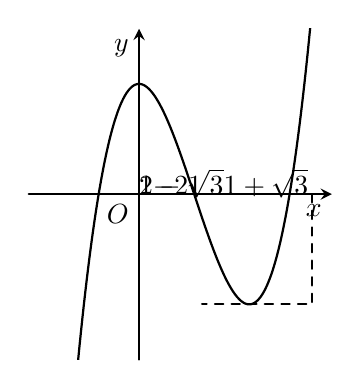
\begin{tikzpicture}[line join=round, line cap=round,>=stealth,thick,scale=.7]
		\def\xmin{-2}
		\def\xmax{3.5}
		\def\ymin{-3}
		\def\ymax{3}
		\tikzset{label style/.style={font=\footnotesize}}
		\draw[->] (\xmin,0)--(\xmax,0) node[below left] {$x$};
		\draw[->] (0,\ymin)--(0,\ymax) node[below left] {$y$};
		\draw (0,0) node [below left] {$O$};
		\begin{scope}
		\clip (\xmin,\ymin) rectangle (\xmax,\ymax); 
		\draw[samples=200,domain=\xmin:\xmax,smooth,variable=\x] plot (\x,{(\x)^3-3*(\x)^2+2});
		
		\tkzLabelPoint[above](2,0){$2$};
		\tkzLabelPoint[left](0,-2){$-2$};
		\tkzLabelPoint[below left](1,0){$1$};
		\draw [dashed](2,0) -- (2,-2)--(0,-2);
		\end{scope}
		\tkzLabelPoint[above left](-0.73,0){$1-\sqrt{3}$};
		\tkzLabelPoint[above right](2.73,0){$1+\sqrt{3}$};
		\end{tikzpicture}
	}
	\loigiai{
		Xét phương trình $\left(x^3-3x^2+2\right)^3-3\left(x^3-3x^2+2\right)^2+2=0 \quad (1)$.\\
		Đặt $t=x^3-3x^2+2$ (*) thì $(1)$ trở thành $t^3-3t^2+2=0 \quad (2)$.\\
		Theo đồ thị ta có $(2)$ có ba nghiệm phân biệt $\hoac{&t=1\\&t=1-\sqrt{3}\\&t=1+\sqrt{3}.}$ \\
		Từ đồ thị hàm số ta có\\
		+ $t=1\in(-2;2)$ (*) có ba nghiệm phân biệt.\\
		+ $t=1-\sqrt{3}\in(-2;2)$ nên (*) có ba nghiệm phân biệt (khác ba nghiệm khi $t=1$).\\
		+ $t=1+\sqrt{3}>2$ nên (*) có đúng một nghiệm.\\
		Vậy phương trình đã cho có 7 nghiệm phân biệt.}
\end{ex}
\begin{ex}%[Nguyễn Tâm Phục]%[2D1K4-3]%Câu 39.
	Tìm tất cả các giá trị thực của tham số $m$ để đồ thị hàm số $y=\dfrac{x+1}{\sqrt{m(x-1)^2+4}}$ có hai tiệm cận đứng.
	\choice
	{$m<0$}
	{$m=0$}
	{\True $\heva{&m<0\\&m\neq-1}$}
	{$m<1$}
	\loigiai{
		Đặt $g(x)=m(x-1)^2+4=mx^2-2mx+4+m$.\\
		Để đồ thị hàm số có hai tiệm cận đứng thì cần tìm $m$ để phương trình $g(x)=0$ có hai nghiệm 	phân biệt khác $-1$.\\
		Điều kiện là $\heva{&m\neq 0\\&\Delta=m^2-m(4+m)>0\\&g(-1)\neq 0}\Leftrightarrow\heva{&m<0\\&m\neq-1}$.}
\end{ex}
\begin{ex}%[Nguyễn Tâm Phục]%[2D1G5-4]%Câu 40.
	Cho hàm số $y=x^3+2mx^2+3(m-1)x+2$ có đồ thị $(C)$. Đường thẳng $d\colon y=-x+2$ cắt đồ thị $(C)$ tại ba điểm phân biệt $A(0;2)$, $B$ và $C$. Với $M(3;1)$, giá trị của tham số $m$ để tam giác $MBC$ có diện tích bằng $2\sqrt{6}$ là
	\choice
	{$m=-1$}
	{\True $m=-1$ hoặc $m=4$}
	{$m=4$}
	{Không tồn tại $m$}
	\loigiai{
		Hoành độ giao điểm của $(C)$ và $d$ là nghiệm của phương trình
		\begin{eqnarray*}
			&&x^3+2mx^2+3(m-1)x+2=-x+2 \\
			& \Leftrightarrow & x^3+2mx^2+(3m-2)x=0  \\
			& \Leftrightarrow & x\left(x^2+2mx+3m-2\right)=0  \\
			& \Leftrightarrow & \hoac{&x=0\\&x^2+2mx+3m-2=0 \quad (*).} 
		\end{eqnarray*}		
		$(C)$ cắt $d$ tại ba điểm phân biệt khi chỉ khi (*) có hai nghiệm phân biệt khác $0$\\
		khi chỉ khi $\heva{&3m-2\neq 0\\&m^2-3m+2>0}\Leftrightarrow\heva{&m\neq\dfrac{2}{3}\\&\hoac{&m<1\\&m>2}}\Leftrightarrow\hoac{&m<1\\&m>2.}$ \\
		Giả sử toạ độ giao điểm của là $A(0;2)$, $B(x_B;y_B), C(x_C;y_C)$ với $x_B; x_C$ là nghiệm của $(*)$.\\
		Khi đó, ta có $\heva{&x_B+x_C=-2m\\&x_B\cdot x_C=3m-2}$ và $\heva{&y_B=-x_B+2\\&y_C=-x_C+2.}$ \\
		Suy ra $BC=\sqrt{2(x_B-x_C)^2}=\sqrt{2\left[(x_B+x_C)^2-4x_Bx_C\right]}=\sqrt{2\left[4m^2-4(3m-2)\right]}$.\\
		Mà $\mathrm{d}(M;d)=\dfrac{|3+1-2|}{\sqrt{1^2+1^2}}=\sqrt{2}$.\\
		Ta có 
		\begin{eqnarray*}
			&&S_{\triangle MBC}=\dfrac{1}{2}\mathrm{d}(M;d)\cdot BC\\ 
			& \Leftrightarrow & \dfrac{1}{2}\cdot\sqrt{2}\cdot\sqrt{2\left[4m^2-4(3m-2)\right]}=2\sqrt{6}\\
			&\Leftrightarrow & 4m^2-4(3m-2)=24 \\
			&\Leftrightarrow & m^2-3m-4=0\\
			& \Leftrightarrow & \hoac{&m=-1\\&m=4}  (\text{thoả mãn } (*))
		\end{eqnarray*}
	}
\end{ex}
\begin{ex}%[Nguyễn Tâm Phục]%[2D1G5-7]%Câu 41.
	Cho hàm số $y=\dfrac{x-3}{x+1} \quad (C)$ và điểm $M(a;b)$ thuộc đồ thị $(C)$. Đặt $T=3(a+b)+2ab$, khi đó để tổng khoảng cách từ điểm $M$ đến hai trục toạ độ là nhỏ nhất thì mệnh đề nào sau đây là đúng?
	\choice
	{\True $-3<T <-1$}
	{$-1<T<1$}
	{$1<T<3$}
	{$2<T<4$}
	\loigiai{
		Hàm số $y=\dfrac{x-3}{x+1}$ có tập xác định: $\mathscr{D}=\mathbb{R}\setminus\{-1\}$.\\
		Điểm $M(a;b)\in(C)\Rightarrow b=\dfrac{a-3}{a+1}(a\neq-1)$.\\
		Trục $Ox$, $Oy$ lần lượt có phương trình là $y=0$ và $x=0$.\\
		Tổng khoảng cách từ $M(a;b)$ đến hai trục tọa độ là $P=\left|\dfrac{a-3}{a+1}\right|+|a|$.\\
		Xét hàm số $P=\left|\dfrac{a-3}{a+1}\right|+|a|$ có tập xác định: $\mathscr{D}=\mathbb{R}\setminus\{-1\}$.\\
		$P=\left|\dfrac{a-3}{a+1}\right|+|a|=\heva{&a+\dfrac{a-3}{a+1} &&\text{khi } a\geq 3\\&a+\dfrac{3-a}{a+1} &&\text{khi } 0<a<3\\&\dfrac{3-a}{a+1}-a &&\text{khi }-1<a\leq 0\\&\dfrac{a-3}{a+1}-a &&\text{khi } a <-1}\Rightarrow P'=\heva{&1+\dfrac{4}{(a+1)^2}&&\text{khi } a\geq 3\\&1-\dfrac{4}{(a+1)^2}&&\text{khi } 0<a<3\\&-\dfrac{4}{(a+1)^2}-1 &&\text{khi }-1<a\leq 0\\&\dfrac{4}{(a+1)^2}-1 &&\text{khi } a <-1.}$ \\
		Bảng biến thiên:
		\begin{center}
			
\begin{tikzpicture}
			\tkzTabInit[espcl=2,lgt=1]
			{$a$/0.7,$P'$/0.7,$P$/2.5}
			{$-\infty$,$-3$,$-1$,$0$,$1$,$3$,$+\infty$}
			\tkzTabLine{,-,0,+,d,-,t,-,0,+,t,+}
			%\tkzTabVar{+/$+\infty$,-/$6$}
			\tkzTabVar{+/$+\infty$,-/$6$,+D+/ $+\infty$/$+\infty$,R/,-/$2$,R/,+/$+\infty$}
			\end{tikzpicture}
		\end{center}
		Vậy $\min(P)=2$ khi $a=1\Rightarrow b=-1$. Do đó $M(1;-1)\Rightarrow T=-2$.}
\end{ex}
\begin{ex}%[Nguyễn Tâm Phục]%[2D1K5-5]%Câu 42.
	\immini{Cho hàm số $y=f(x)$. Đồ thị của hàm số $y=f'(x)$ như hình vẽ. Đặt $h(x)=f(x)-x$. Mệnh đề nào dưới đây đúng?
		
		\choice
		{$h(1)+1=h(4)<h(2)$}
		{$h(0)=h(4)+2<h(2)$}
		{\True $h(-1)<h(0)<h(2)$}
		{$h(2)<h(4)<h(0)$}
	}{
		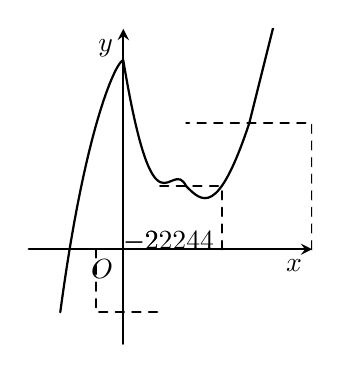
\begin{tikzpicture}[line join=round, line cap=round,>=stealth,thick,scale=.4]
		\def\xmin{-3}
		\def\xmax{6}
		\def\ymin{-3}
		\def\ymax{7}
		\tikzset{label style/.style={font=\footnotesize}}
		\draw[->] (\xmin,0)--(\xmax,0) node[below left] {$x$};
		\draw[->] (0,\ymin)--(0,\ymax) node[below left] {$y$};
		\draw (0,0) node [below left] {$O$};
		\begin{scope}
		\clip (\xmin,\ymin) rectangle (\xmax,\ymax); 
		
		\draw   (-2,-2) .. controls (-1.2,4) and (-0.2,6) .. (0,6);
		\draw   (0,6) .. controls (1,0) and (1.5,3) .. (2,2);
		\draw   (2,2) .. controls (2.5,1.5) and (3,1) .. (4,4);
		\draw (4,4) -- (5,8);
		\tkzDrawPoint[fill=black,size=2pt](4,4);
		\tkzDrawPoint[fill=black,size=2pt](-2,-2);
		\tkzLabelPoint[above left](-2,0){$-2$};
		
		\draw [dashed](-2,0) -- (-2,-2)--(0,-2);
		\tkzDrawPoint[fill=black,size=2pt](2,2);
		\draw [dashed](2,0) -- (2,2)--(0,2);
		\tkzLabelPoint[left](0,2){$2$};
		\tkzLabelPoint[below](2,0){$2$};
		\draw [dashed](4,0) -- (4,4)--(0,4);
		\tkzLabelPoint[below](4,0){$4$};
		\tkzLabelPoint[left](0,4){$4$};
		\end{scope}
		\tkzLabelPoint[right](0,-2){$-2$};
		\end{tikzpicture}
	}
	\loigiai{
		Xét hàm số $h(x)=f(x)-x$ trên đoạn $[-1;4]$.\\
		Ta có $h'(x)=f'(x)-1$. Dựa vào đồ thị của hàm số $y=f'(x)$ trên đoạn $[-1;4]$ ta được $h'(x)>0$. Suy ra hàm số đồng biến trên $[-1;4]$. }
\end{ex}
\begin{ex}%[Nguyễn Tâm Phục]%[2D1K5-3]%Câu 43.
	Tìm tất cả giá trị thực của tham số $m$ để phương trình $\left|x^3-3x^2+2\right|-m=1$ có $6$ nghiệm phân biệt. 
	\choice
	{$1<m<3$}
	{$-2<m<0$}
	{\True $-1<m<1$}
	{$0<m<2$}
	\loigiai{
		
		$\left|x^3-3x^2+2\right|-m=1\Leftrightarrow\left|x^3-3x^2+2\right|=m+1$.\\
		Xét hàm số $y=x^3-3x^2+2$.\\
		$y'=3x^2-6x; y'=0\Leftrightarrow\hoac{&x=0\\&x=2.}$ \\
		Đồ thị hàm số $y=x^3-3x^2+2$.\\
		\begin{center}
			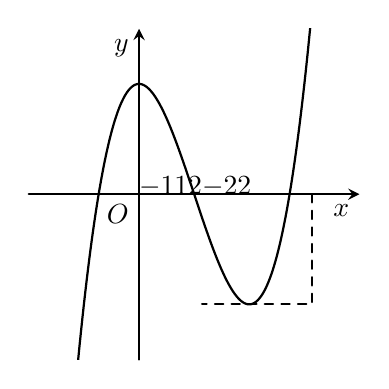
\begin{tikzpicture}[line join=round, line cap=round,>=stealth,thick,scale=.7]
			\def\xmin{-2}
			\def\xmax{4}
			\def\ymin{-3}
			\def\ymax{3}
			\tikzset{label style/.style={font=\footnotesize}}
			\draw[->] (\xmin,0)--(\xmax,0) node[below left] {$x$};
			\draw[->] (0,\ymin)--(0,\ymax) node[below left] {$y$};
			\draw (0,0) node [below left] {$O$};
			\begin{scope}
			\clip (\xmin,\ymin) rectangle (\xmax,\ymax); 
			\draw[samples=200,domain=\xmin:\xmax,smooth,variable=\x] plot (\x,{(\x)^3-3*(\x)^2+2});
			\tkzDrawPoint[fill=black,size=2pt](-1,0);
			\tkzLabelPoint[above](-1,0){$-1$};			
			\tkzDrawPoint[fill=black,size=2pt](2,0);
			\tkzLabelPoint[above right](1,0){$1$};
			\tkzLabelPoint[above](2,0){$2$};
			\draw [dashed](2,0) -- (2,-2)--(0,-2);
			\tkzLabelPoint[left](0,-2){$-2$};
			\tkzLabelPoint[above right](0,2){$2$};
			\end{scope}
			\end{tikzpicture}
		\end{center}
		Từ đó ta suy ra đồ thị hàm số $y=\left|x^3-3x^2+2\right|$. 
		\begin{center}
			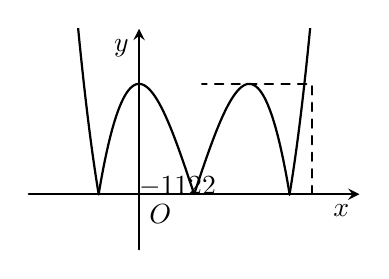
\begin{tikzpicture}[line join=round, line cap=round,>=stealth,thick,scale=.7]
			\def\xmin{-2}
			\def\xmax{4}
			\def\ymin{-1}
			\def\ymax{3}
			\tikzset{label style/.style={font=\footnotesize}}
			\draw[->] (\xmin,0)--(\xmax,0) node[below left] {$x$};
			\draw[->] (0,\ymin)--(0,\ymax) node[below left] {$y$};
			\draw (0,0) node [below right] {$O$};
			\begin{scope}
			\clip (\xmin,\ymin) rectangle (\xmax,\ymax); 
			\draw[samples=200,domain=-0.73:1,smooth,variable=\x] plot (\x,{(\x)^3-3*(\x)^2+2});
			\draw[samples=200,domain=2.73:\xmax,smooth,variable=\x] plot (\x,{(\x)^3-3*(\x)^2+2});
			\draw[samples=200,domain=\xmin:-0.73,smooth,variable=\x] plot (\x,{-(\x)^3+3*(\x)^2-2});
			\draw[samples=200,domain=1:2.73,smooth,variable=\x] plot (\x,{-(\x)^3+3*(\x)^2-2});
			\tkzDrawPoint[fill=black,size=2pt](-1,0);
			\tkzLabelPoint[below](-1,0){$-1$};			
			\tkzDrawPoint[fill=black,size=2pt](2,0);
			\tkzLabelPoint[below](1,0){$1$};
			\tkzLabelPoint[below](2,0){$2$};
			\draw [dashed](2,0) -- (2,2)--(0,2);			
			\tkzLabelPoint[above right](0,2){$2$};
			\end{scope}
			\end{tikzpicture}
		\end{center}
		Số nghiệm của phương trình $\left|x^3-3x^2+2\right|-m=1$ là hoành độ giao điểm của đồ thi hàm số $y=\left|x^3-3x^2+2\right|$ và đường thẳng $y=m+1$.\\
		Nhìn vào đồ thị ta thấy để phương trình có 6 nghiệm cần: $0<m+1<2\Leftrightarrow-1<m<1$.}
\end{ex}
\begin{ex}%[Nguyễn Tâm Phục]%[2D1G3-6]%Câu 44.
	\immini{Một cái ao hình $ABCDE$ (như hình vẽ), ở giữa ao có một mảnh vườn hình tròn có bán kính $10$ m. Người ta muốn bắc một câu cầu từ bờ $AB$ của ao đến vườn. Tính gần đúng độ dài tối thiếu $l$ của cây cầu biết:\\
		- Hai bờ $AE$ và $BC$ nằm trên hai đường thẳng vuông góc với nhau, hai đường thẳng này cắt nhau tại điểm $O$;\\
		- Bờ $AB$ là một phần của một parabol có đỉnh là điểm $A$ và có trục đối xứng là đường thẳng $OA$;\\
		- Độ dài đoạn $OA$ và $OB$ lần lượt là $40$ m và $20$ m;\\
		- Tâm $I$ của mảnh vườn lần lượt cách đường thẳng $AE$ và $BC$ lần lượt $40$ m và $30$ m. 	
		\choice
		{\True $l\approx 17,7$ m}
		{$l\approx 25,7$ m}
		{$l\approx 27,7$ m}
		{$l\approx 15,7$ m}
	}{
		\begin{tikzpicture}[line join=round, line cap=round,>=stealth,thick,scale=.6]
		\def\xmin{0}
		\def\xmax{8}
		\def\ymin{0}
		\def\ymax{7}
		\tikzset{label style/.style={font=\footnotesize}}			
		\draw (0,0) node [below left] {$O$};
		\begin{scope}
		\clip (\xmin,\ymin) rectangle (\xmax,\ymax); 
		\draw[samples=200,domain=0:2,smooth,variable=\x] plot (\x,{4-(\x)^2});
		\tkzDefPoints{4/3/I,4/2/I'}
		\draw (2,0)--(7,0)--(7,6)--(0,6)--(0,4);
		\draw[pattern =dots, line width = 1.2pt,draw=none] plot[domain=0:2] (\x, {4-(\x)^2})--(2,0)--(7,0)--(7,6)--(0,6)--(0,2);
		\tkzDrawCircle[color=blue!30,fill=blue!30](I,I')
		\draw [dashed](4,0) -- (4,3)--(0,3);
		\tkzDrawPoint[fill=black,size=4pt](4,3);
		\tkzLabelPoint[above](4,3){$I$};
		\draw [dashed](0,4) -- (0,0)--(2,0);
		
		\tkzLabelPoint[above,fill=white](2,3){$40 $ m};
		\tkzLabelPoint[right,fill=white](4,1){$30 $ m};
		\tkzLabelPoint[above](1,0){$20$ m};
		\draw [line width = 2pt] (1.41,1.95) -- (3.08,2.63);
		\end{scope}
		\tkzLabelPoint[left](0,2){$40 $ m};			
		\tkzLabelPoint[left](0,4){$A$};
		\tkzLabelPoint[below](2,0){$B$};
		\tkzLabelPoint[below](7,0){$C$};
		\tkzLabelPoint[right](7,6){$D$};
		\tkzLabelPoint[left](0,6){$E$};
		\end{tikzpicture}
	}
	\loigiai{
		\begin{center}
			\begin{tikzpicture}[line join=round, line cap=round,>=stealth,thick,scale=.6]
			\def\xmin{0}
			\def\xmax{8}
			\def\ymin{0}
			\def\ymax{7}
			\tikzset{label style/.style={font=\footnotesize}}
			\draw[->] (\xmin,0)--(\xmax,0) node[below left] {$x$};
			\draw[->] (0,\ymin)--(0,\ymax) node[below left] {$y$};
			\draw (0,0) node [below left] {$O$};
			\begin{scope}
			\clip (\xmin,\ymin) rectangle (\xmax,\ymax); 
			\draw[samples=200,domain=0:2,smooth,variable=\x] plot (\x,{4-(\x)^2});
			\tkzDefPoints{4/3/I,4/2/I'}
			\draw (2,0)--(7,0)--(7,6)--(0,6)--(0,4);
			\draw[pattern =dots, line width = 1.2pt,draw=none] plot[domain=0:2] (\x, {4-(\x)^2})--(2,0)--(7,0)--(7,6)--(0,6)--(0,2);
			\tkzDrawCircle[color=blue!30,fill=blue!30](I,I')
			\draw [dashed](4,0) -- (4,3)--(0,3);
			\tkzDrawPoint[fill=black,size=4pt](4,3);
			\tkzLabelPoint[above](4,3){$I$};
			\draw [dashed](0,4) -- (0,0)--(2,0);
			
			\tkzLabelPoint[above,fill=white](2,3){$40 $ m};
			\tkzLabelPoint[right,fill=white](4,1){$30 $ m};
			\tkzLabelPoint[above](1,0){$20$ m};
			\draw [line width = 2pt] (1.41,1.95) -- (3.08,2.63);
			\end{scope}
			\tkzLabelPoint[left](0,2){$40 $ m};
			\tkzLabelPoint[left](0,3){$3$};
			\tkzLabelPoint[left](0,4){$A$};
			\tkzLabelPoint[below](2,0){$B$};
			\tkzLabelPoint[below](7,0){$C$};
			\tkzLabelPoint[right](7,6){$D$};
			\tkzLabelPoint[left](0,6){$E$};
			\end{tikzpicture}
		\end{center}
		Gán trục tọa độ $Oxy$ sao cho $\heva{&A\in Oy\\&B\in Ox}$ cho đơn vị là $10$ m.\\
		Khi đó mảnh vườn hình tròn có phương trình $(C)\colon (x-4)^2+(y-3)^2=1$ có tâm $I(4;3)$.\\
		Bờ $AB$ là một phần của Parabol $(P)\colon y=4-x^2$ ứng với $x\in[0;2]$.\\
		Vậy bài toán trở thành tìm $MN$ nhỏ nhất với $\heva{&M\in(P)\\&N\in(C).}$ \\
		Đặt trường hợp khi đã xác định được điểm $N$ thì $MN+MI\geq IM$, vậy $MN$ nhỏ nhất khi $MN+MI=IM\Leftrightarrow N$; $M$; $I$ thẳng hàng.\\
		Bây giờ, ta sẽ xác định điểm $N$ để $IN$ nhỏ nhất.\\
		$N\in(P)\Leftrightarrow N\left(x;4-x^2\right) IN=\sqrt{(4-x)^2+\left(1-x^2\right)^2}\Leftrightarrow IN^2=(4-x)^2+\left(1-x^2\right)^2$ \\
		$ \Leftrightarrow IN^2=x^4-x^2-8x+17 $.\\
		Xét $f(x)=x^4-x^2-8x+17$ trên $[0;2]\Leftrightarrow f'(x)=4x^3-2x-8$.\\
		$f'(x)=0\Leftrightarrow x\approx 1,3917$ là nghiệm duy nhất và $1,3917\in[0;2]$.\\
		Ta có $f(1,3917)=7,68$; $f(0)=17$; $f(2)=13$.\\
		Vậy giá trị nhỏ nhất của $f(x)$ trên $[0;2]$ gần bằng $7,68$ khi $x\approx 1,3917$.\\
		Vậy $\min IN\approx\sqrt{7,68}\approx 2,77\Leftrightarrow IN=27,7$ m $\Leftrightarrow MN=IN-IM=27,7-10=17,7$ m.}
\end{ex}
\begin{ex}%[Nguyễn Tâm Phục]%[2D1G5-5]%Câu 45.
	\immini{Cho hàm số $y=f(x)$ có đồ thị $f'(x)$ như hình vẽ.	
		Hàm số $y=f(1-x)+\dfrac{x^2}{2}-x$ nghịch biến trên khoảng
		\choice
		{$(-3; 1)$}
		{$(-2; 0)$}
		{\True $(1; 3)$}
		{$\left(-1;\dfrac{3}{2}\right)$}
	}{
		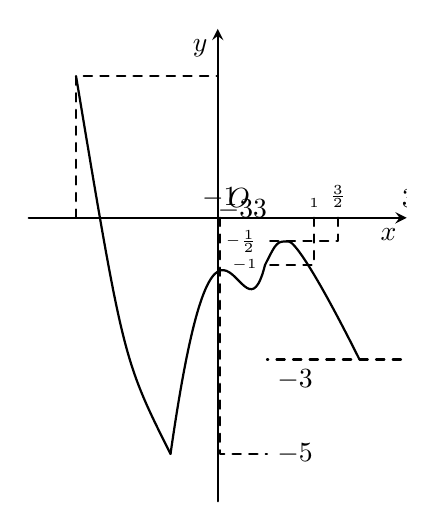
\begin{tikzpicture}[line join=round, line cap=round,>=stealth,thick,scale=.6]
		\def\xmin{-4}
		\def\xmax{4}
		\def\ymin{-6}
		\def\ymax{4}
		\tikzset{label style/.style={font=\footnotesize}}
		\draw[->] (\xmin,0)--(\xmax,0) node[below left] {$x$};
		\draw[->] (0,\ymin)--(0,\ymax) node[below left] {$y$};
		\draw (0,0) node [above right] {$O$};
		\begin{scope}
		\clip (\xmin,\ymin) rectangle (\xmax,\ymax); 
		\draw   (-3,3) .. controls (-2,-3) .. (-1,-5);
		\draw   (-1,-5) .. controls (0,2) and (0.5,-3) .. (1,-1);
		\draw   (1,-1) .. controls (1.25,-0.5).. (1.5,-0.5);
		\draw   (1.5,-0.5) .. controls (1.6,-0.5) and  (2,-1).. (3,-3);
		\draw [dashed](-3,0) -- (-3,3)--(0,3);
		\tkzLabelPoint[below](-3,0){$-3$};
		\tkzLabelPoint[right](0,3){$3$};
		\draw [dashed](-1,0) node[above]{$-1$}-- (-1,-5)--(0,-5) node[right]{$-5$};
		\draw [dashed](1,0) node[above]{\tiny $1$}-- (1,-1)--(0,-1) node [left]{\tiny $-1$};
		\draw [dashed](1.5,0) node[above]{\tiny $\frac{3}{2}$} -- (1.5,-0.5)--(0,-0.5)node[left]{\tiny $-\frac{1}{2}$};
		\draw [dashed](3,0) node[above]{$3$} -- (3,-3)--(0,-3)node[below right]{$-3$};
		\end{scope}
		\end{tikzpicture}
	}
	\loigiai{
		\begin{center}
			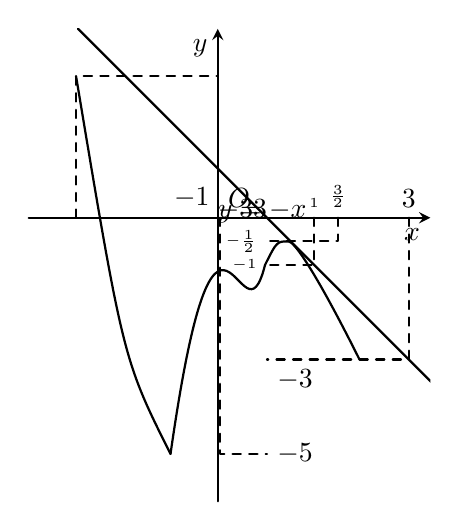
\begin{tikzpicture}[line join=round, line cap=round,>=stealth,thick,scale=.6]
			\def\xmin{-4}
			\def\xmax{4.5}
			\def\ymin{-6}
			\def\ymax{4}
			\tikzset{label style/.style={font=\footnotesize}}
			\draw[->] (\xmin,0)--(\xmax,0) node[below left] {$x$};
			\draw[->] (0,\ymin)--(0,\ymax) node[below left] {$y$};
			\draw (0,0) node [above right] {$O$};
			\begin{scope}
			\clip (\xmin,\ymin) rectangle (\xmax,\ymax); 
			\draw   (-3,3) .. controls (-2,-3) .. (-1,-5);
			\draw   (-1,-5) .. controls (0,2) and (0.5,-3) .. (1,-1);
			\draw   (1,-1) .. controls (1.25,-0.5).. (1.5,-0.5);
			\draw   (1.5,-0.5) .. controls (1.6,-0.5) and  (2,-1).. (3,-3);
			\draw [dashed](-3,0) -- (-3,3)--(0,3);
			\tkzLabelPoint[below](-3,0){$-3$};
			\tkzLabelPoint[right](0,3){$3$};
			\draw [dashed](-1,0) node[above left]{$-1$}-- (-1,-5)--(0,-5) node[right]{$-5$};
			\draw [dashed](1,0) node[above]{\tiny $1$}-- (1,-1)--(0,-1) node [left]{\tiny $-1$};
			\draw [dashed](1.5,0) node[above]{\tiny $\frac{3}{2}$} -- (1.5,-0.5)--(0,-0.5)node[left]{\tiny $-\frac{1}{2}$};
			\draw [dashed](3,0) node[above]{$3$} -- (3,-3)--(0,-3)node[below right]{$-3$};
			\draw[samples=200,domain=\xmin:\xmax,smooth,variable=\x] plot (\x,{-1*(\x)});			
			\end{scope}
			\tkzLabelPoint[right](3,-5){$y=-x$};
			\end{tikzpicture}
		\end{center}
		Xét hàm số $y=f(1-x)+\dfrac{x^2}{2}-x$ có $y'=-f'(1-x)+x-1$.\\
		$y'=0\Leftrightarrow-f'(1-x)+x-1=0\Leftrightarrow f'(1-x)=-(1-x)\Leftrightarrow\hoac{&1-x=-3\\&1-x=1\\&1-x=3}\Leftrightarrow\hoac{&x=4\\&x=0\\&x=-2.}$ \\
		Ta có bảng biến thiên: 
		\begin{center}
			
\begin{tikzpicture}
			\tkzTabInit[espcl=2.3,lgt=1.5]
			{$x$/0.7,$y'$/0.7,$y$/2.3}
			{$-\infty$,$-2$,0,$4$,$+\infty$}
			\tkzTabLine{,-,0,+,0,-,0,+}
			\tkzTabVar{+/$+\infty$,-/,+/,-/,+/$+\infty$}
			\end{tikzpicture}
		\end{center}
		Do đó Hàm số $y=f(1-x)+\dfrac{x^2}{2}-x$ nghịch biến trên khoảng $(1;3)$.}
\end{ex}
\begin{ex}%[Nguyễn Tâm Phục]%[2D1G2-6]%Câu 46.
	Có bao nhiêu giá trị nguyên dương của tham số $m$ để hàm số\break $y=\left|3x^4-4x^3-12x^2+m\right|$ có $5$ điểm cực trị. 
	\choice
	{$44$}
	{\True $27$}
	{$26$}
	{$16$}
	\loigiai{
		Xét hàm số $f(x)=3x^4-4x^3-12x^2+m$.\\
		Ta có $f'(x)=12x^3-12x^2-24x$,\\
		$f'(x)=0\Leftrightarrow 12x^3-12x^2-24x=0\Leftrightarrow\hoac{&x=0\\&x=-1\\&x=2.}$ \\
		Ta có bảng biến thiên
		\begin{center}
			
\begin{tikzpicture}
			\tkzTabInit[espcl=2.3,lgt=1.5]
			{$x$/0.7,$f'(x)$/0.7,$f(x)$/2.3}
			{$-\infty$,$-1$,0,$2$,$+\infty$}
			\tkzTabLine{,-,0,+,0,-,0,+}
			\tkzTabVar{+/$+\infty$,-/$m-5$,+/$m$,-/$m-32$,+/$+\infty$}
			\end{tikzpicture}
		\end{center}
		Xét hàm số $y=\left|f(x)\right|=\heva{&f(x) &&\text{nếu } f(x)\geq 0\\&-f(x) &&\text{nếu } f(x)<0.}$ \\
		Nên từ bảng biến thiên của hàm số $y=f(x)$ suy ra hàm số $y=\left|3x^4-4x^3-12x^2+m\right|$ có $5$ điểm cực trị khi và chỉ khi $\heva{&m-32<0\\&m-5\geq 0}\Leftrightarrow 5\leq m<32$.\\
		Do đó có $27$ giá trị nguyên dương của tham số $m$ để hàm số $y=\left|3x^4-4x^3-12x^2+m\right|$ có $5$ điểm cực trị.}
\end{ex}
\begin{ex}%[Nguyễn Tâm Phục]%[2D1G5-5]%Câu 47.
	\immini{Cho hàm số $y=f(x)$ có đạo hàm liên tục trên đoạn $[-3;3]$ và đồ thị hàm số $y=f'(x)$ như hình vẽ bên. Biết $f(1)=6$ và $g(x)=f(x)-\dfrac{(x+1)^2}{2}$. Kết luận nào sau đây là đúng?
		\choice
		{Phương trình $g(x)=0$ có đúng hai nghiệm thuộc $[-3;3]$}
		{Phương trình $g(x)=0$ không có nghiệm thuộc $[-3;3]$.\\
		}
		{\True Phương trình $g(x)=0$ có đúng một nghiệm thuộc $[-3;3]$}
		{Phương trình $g(x)=0$ có đúng ba nghiệm thuộc $[-3;3]$}
	}{
		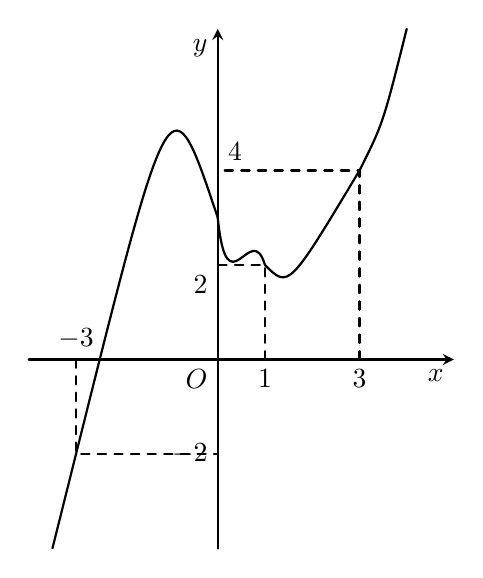
\begin{tikzpicture}[line join=round, line cap=round,>=stealth,thick,scale=.6]
		\def\xmin{-4}
		\def\xmax{5}
		\def\ymin{-4}
		\def\ymax{7}
		\tikzset{label style/.style={font=\footnotesize}}
		\draw[->] (\xmin,0)--(\xmax,0) node[below left] {$x$};
		\draw[->] (0,\ymin)--(0,\ymax) node[below left] {$y$};
		\draw (0,0) node [below left] {$O$};
		\begin{scope}
		\clip (\xmin,\ymin) rectangle (\xmax,\ymax); 
		\draw   (-3,-2) .. controls (-1,6) .. (0,3);
		\draw   (0,3) .. controls (0.2,1) and (0.7,3) .. (1,2);
		\draw   (1,2) .. controls (1.5,1.5)  .. (3,4);
		\draw (-3.5,-4) -- (-3,-2);
		:\draw (3,4) .. controls (3.5,5.0) .. (4,7);
		\draw [dashed](-3,0) node [above]{$-3$} -- (-3,-2)--(0,-2)node[left]{$-2$};
		\draw [dashed](1,0) node[below]{$1$} -- (1,2)--(0,2) node[below left]{$2$};
		\draw [dashed](3,0) node[below]{$3$} -- (3,4)--(0,4)node[above right]{$4$};
		\end{scope}
		\end{tikzpicture}
	}
	\loigiai{
		\begin{center}
			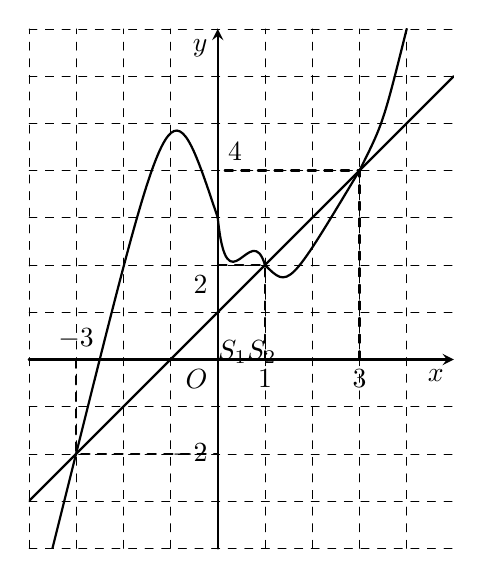
\begin{tikzpicture}[line join=round, line cap=round,>=stealth,thick,scale=.6]
			\def\xmin{-4}
			\def\xmax{5}
			\def\ymin{-4}
			\def\ymax{7}
			\tikzset{label style/.style={font=\footnotesize}}
			\draw[->] (\xmin,0)--(\xmax,0) node[below left] {$x$};
			\draw[->] (0,\ymin)--(0,\ymax) node[below left] {$y$};
			\draw (0,0) node [below left] {$O$};
			\begin{scope}
			\clip (\xmin,\ymin) rectangle (\xmax,\ymax); 
			\draw[line width=0.2pt,dashed] (\xmin,\ymin) grid (\xmax,\ymax);
			\draw   (-3,-2) .. controls (-1,6) .. (0,3);
			\draw   (0,3) .. controls (0.2,1) and (0.7,3) .. (1,2);
			\draw   (1,2) .. controls (1.5,1.5)  .. (3,4);
			\draw (-3.5,-4) -- (-3,-2);
			:\draw (3,4) .. controls (3.5,5.0) .. (4,7);
			\draw [dashed](-3,0) node [above]{$-3$} -- (-3,-2)--(0,-2)node[left]{$-2$};
			\draw [dashed](1,0) node[below]{$1$} -- (1,2)--(0,2) node[below left]{$2$};
			\draw [dashed](3,0) node[below]{$3$} -- (3,4)--(0,4)node[above right]{$4$};
			\draw[samples=200,domain=\xmin:\xmax,smooth,variable=\x] plot (\x,{(\x)+1});
			\tkzLabelPoint[above](-1.5,1){$S_1$};
			\tkzLabelPoint[right](1,2){$S_2$};
			\end{scope}
			\end{tikzpicture}
		\end{center}
		Ta có: $g(x)=f(x)-\dfrac{(x+1)^2}{2}\Rightarrow g'(x)=f'(x)-(x+1)$.\\
		Vẽ đường thẳng $y=x+1$ trên cùng một hệ trục tọa độ với đồ thị hàm số $y=f'(x)$ (như hình vẽ bên).\\
		Từ đồ thị ta thấy: $g'(x)=f'(x)-(x+1)>0$, $\forall x\in(-3;1)$ (do đường cong nằm phía trên đường thẳng), $g'(x)=f'(x)-(x+1)<0$, $\forall x\in(1;3)$ (do đường cong nằm phía dưới đường thẳng).\\
		Ta có: $g(1)=f(1)-\dfrac{(1+1)^2}{2} =6-2=4$.\\
		Bảng biến thiên: 
		\begin{center}
			
\begin{tikzpicture}
			\tkzTabInit[espcl=2.3,lgt=1]
			{$x$/0.7,$g'(x)$/0.7,$g(x)$/2.3}
			{$-3$,$1$,$3$}
			\tkzTabLine{,+,0,-}
			\tkzTabVar{-/,+/$4$,-/}
			\end{tikzpicture}
		\end{center}
		Dựa vào đồ thị ta thấy: diện tích $S_1$ lớn hơn $4$ (trong phần bên trái có nhiều hơn 4 ô, mỗi ô có diện tích bằng $1$), do đó:\\
		$4<S_1=\displaystyle\int\limits_{-3}^1 g'(x)\mathrm{\,d}x\Leftrightarrow 4< g(x)\bigg|_{-3}^1\Leftrightarrow 4<g(1)-g(-3)\Leftrightarrow g(-3)<0$.\\
		Mặt khác: diện tích nhỏ hơn $4$ (trong phần bên phải có ít hơn $4$ ô), do đó:\\
		$4>S_2=-\displaystyle\int\limits_1^3 g'(x)\mathrm{\,d}x\Leftrightarrow 4 >- g(x)\bigg|_1^3\Leftrightarrow 4>g(1)-g(3)\Leftrightarrow g(3)>0$.\\
		Vậy phương trình $g(x)=0$ có đúng một nghiệm thuộc đoạn $[-3;3]$ (nghiệm này nằm trong khoảng $(-3;1)$).}
\end{ex}
\begin{ex}%[Nguyễn Tâm Phục]%[2D1G1-4]%Câu 48.
	Phương trình $\sqrt{x-512}+\sqrt{1024-x}=16+4\sqrt[8]{(x-512)(1024-x)}$ có bao nhiêu nghiệm?
	\choice
	{$4$ nghiệm}
	{\True $3$ nghiệm}
	{$8$ nghiệm}
	{$2$ nghiệm}
	\loigiai{
		Phương trình $\sqrt{x-512}+\sqrt{1024-x}=16+4\sqrt[8]{(x-512)(1024-x)} \quad (1)$.\\
		Điều kiện: $x\in[512; 1024]$.\\
		Bình phương hai vế của phương trình $(1)$ ta có:\\
		$512+2\sqrt{(x-512)(1024-x)}=256+128\sqrt[8]{(x-512)(1024-x)}+16\sqrt[4]{(x-512)(1024-x)} \quad (2)$.\\
		Đặt $t=\sqrt[8]{(x-512)(1024-x)}$ điều kiện $0\leq t\leq 4$.\\
		$(2)$ trở thành $t^4-8t^2-64t+128=0\Leftrightarrow(t-4)\left(t^3+4t^2+8t-32\right)=0$ \\
		$ \Leftrightarrow\hoac{&t=4\\&t^3+4t^2+8t-32=0.} $ \\
		+ Với $t=4$, mà theo trên ta có $t\leq 4$. Do đó đẳng thức xảy ra khi và chỉ khi $x-512=1024-x\Leftrightarrow x=768$.\\
		+ Với $t^3+4t^2+8t-32=0$.\\
		Xét hàm số $f(t)=t^3+4t^2+8t-32$ với $0\leq t\leq 4$.\\
		Ta có $f'(t)=3t^2+8t+8>0\forall t\in[0; 4]$.\\
		Mà $f(0)\cdot f(4)=-32\cdot 128<0$.\\
		Suy ra $t^3+4t^2+8t-32=0$ có một nghiệm duy nhất $t_0$ trong khoảng $(0; 4)$.\\
		Do đó phương trình $\sqrt[8]{(x-512)(1024-x)}=t_0$ có $2$ nghiệm phân biệt khác $768$.\\
		Vậy phương trình $(1)$ có $3$ nghiệm.}
\end{ex}
\begin{ex}%[Nguyễn Tâm Phục]%[2D1G5-5]%Câu 49.
	Cho phương trình:\\
	$\sin x(2-\cos 2x)-2\left(2\cos^3x+m+1\right)\sqrt{2\cos^3x+m+2}=3\sqrt{2\cos^3x+m+2}$.\\
	Có bao nhiêu giá trị nguyên của tham số $m$ để phương trình trên có đúng $1$ nghiệm $x\in\left[0;\dfrac{2\pi}{3}\right)$?
	\choice
	{$2$}
	{$1$}
	{$4$}
	{\True $3$}
	\loigiai{
		Ta có:\\
		$\sin x(2-\cos 2x)-2\left(2\cos^3x+m+1\right)\sqrt{2\cos^3x+m+2}=3\sqrt{2\cos^3x+m+2}$ \\
		$ \Leftrightarrow\sin x\left(1+2\sin^2x\right)=2\left(2\cos^3x+m+2\right)\sqrt{2\cos^3x+m+2}+\sqrt{2\cos^3x+m+2} $ \\
		$ \Leftrightarrow 2\sin^3x+\sin x=2\left(\sqrt{2\cos^3x+m+2}\right)^3+\sqrt{2\cos^3x+m+2}\quad(1) $.\\
		Xét hàm số $f(t)=2t^3+t$ có $f'(t)=6t^2+1>0,\forall t\in\mathbb{R}$, nên hàm số $f(t)$ đồng biến trên $\mathbb{R}$.\\
		Bởi vậy:\\
		$(1)\Leftrightarrow f(\sin x)=f\left(\sqrt{2\cos^3x+m+2}\right)\Leftrightarrow\sin x=\sqrt{2\cos^3x+m+2}\quad(2)$.\\
		Với $x\in\left[0;\dfrac{2\pi}{3}\right)$ thì\\
		$(2)\Leftrightarrow\sin^2x=2\cos^3x+m+2$ \\
		$ \Leftrightarrow-2\cos^3x-\cos^2x-1=m(3) $.\\
		Đặt $t=\cos x$, phương trình $(3)$ trở thành $-2t^3-t^2-1=m(4)$.\\
		Ta thấy, với mỗi $t\in\left(-\dfrac{1}{2};1\right]$ thì phương trình $\cos x=t$ cho ta một nghiệm $x\in\left[0;\dfrac{2\pi}{3}\right)$. Do đó, để phương trình đã cho có đúng $1$ nghiệm $x\in\left[0;\dfrac{2\pi}{3}\right)$ điều kiện cần và đủ là phương trình $(4)$ có đúng một nghiệm $t\in\left(-\dfrac{1}{2};1\right]$.\\
		Xét hàm số $g(t)=-2t^3-t^2-1$ với $t\in\left(-\dfrac{1}{2};1\right]$.\\
		Ta có $g'(t)=-6t^2-2t$, $g'(t)=0\Leftrightarrow\hoac{&t=0\\&t=-\dfrac{1}{3}.}$ \\
		Ta có bảng biến thiên
		\begin{center}
			
\begin{tikzpicture}
			\tkzTabInit[espcl=2.5,lgt=1]
			{$x$/1.2,$y'$/0.7,$y$/2.3}
			{$-\dfrac{1}{2}$,$-\dfrac{1}{3}$,$0$,$1$}
			\tkzTabLine{,-,0,+,0,-,}
			\tkzTabVar{+/$-1$,-/$\dfrac{28}{7}$,+/$-1$,-/$-4$}
			\end{tikzpicture}
		\end{center}
		Từ bảng biến thiên suy ra, phương trình $(4)$ có đúng một nghiệm $t\in\left(-\dfrac{1}{2};1\right]$ khi và chỉ khi $-4\leq m <-\dfrac{28}{27}$.\\
		Hay, các giá trị nguyên của $m$ để phương trình trên có đúng $1$ nghiệm $x\in\left[0;\dfrac{2\pi}{3}\right)$ là $\{-4;-3;-2\}$.}
\end{ex}
\begin{ex}%[Nguyễn Tâm Phục]%[2D1G5-5]%Câu 50.
	\immini{Cho hàm số $y=f(x)$. Hàm số $y=f'(x)$ có đồ thị như hình bên. Hàm số $y=f\left(x-x^2\right)$ nghịch biến trên khoảng nào dưới đây.	
		\choice
		{$\left(-\dfrac{1}{2};+\infty\right)$}
		{$\left(-\dfrac{3}{2};+\infty\right)$}
		{$\left(-\infty;\dfrac{3}{2}\right)$}
		{\True $\left(\dfrac{1}{2};+\infty\right)$}
	}{
		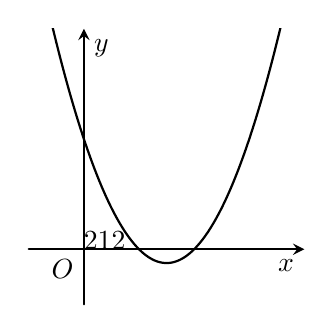
\begin{tikzpicture}[line join=round, line cap=round,>=stealth,thick,scale=.7]
		\def\xmin{-1}
		\def\xmax{4}
		\def\ymin{-1}
		\def\ymax{4}
		\tikzset{label style/.style={font=\footnotesize}}
		\draw[->] (\xmin,0)--(\xmax,0) node[below left] {$x$};
		\draw[->] (0,\ymin)--(0,\ymax) node[below right] {$y$};
		\draw (0,0) node [below left] {$O$};
		
		\begin{scope}
		\clip (\xmin,\ymin) rectangle (\xmax,\ymax);
		\draw[samples=200,domain=\xmin:\xmax,smooth,variable=\x] plot (\x,{(\x)^2-3*(\x)+2});
		\tkzLabelPoint[left](0,2){$2$};
		\tkzLabelPoint[below](1,0){$1$};
		\tkzLabelPoint[below](2,0){$2$};
		\end{scope}
		\end{tikzpicture}
	}
	\loigiai{
		Đặt $y=g(x)=f\left(x-x^2\right)\Rightarrow g'(x)=f'\left(x-x^2\right)\cdot\left(x-x^2\right)'=(1-2x)f'\left(x-x^2\right)$.\\
		Cho $g'(x)=0\Rightarrow\hoac{&1-2x=0\\&f'\left(x-x^2\right)=0}\Rightarrow\hoac{&1-2x=0\\&x-x^2=1(\text { vô nghiệm})\\&x-x^2=2(\text { vô nghiệm})}\Leftrightarrow x=\dfrac{1}{2.}$ \\
		Với $x<\dfrac{1}{2}$ thì $\heva{&1-2x>0\\&f'\left[-\left(x-\dfrac{1}{2}\right)^2+\dfrac{1}{4}\right]>0}$ nên $g'(x)>0$.\\
		Với $x>\dfrac{1}{2}$ thì $\heva{&1-2x<0\\&f'\left[-\left(x-\dfrac{1}{2}\right)^2+\dfrac{1}{4}\right]>0}$ nên $g'(x)<0$ hay hàm số $g(x)=f\left(x-x^2\right)$ nghịch biến trên khoảng $\left(\dfrac{1}{2};+\infty\right)$.}
\end{ex}
\Closesolutionfile{ans}